\documentclass[paper=a4,11pt,titlepage,twoside=true,headings=normal,numbers=noenddot,captions=tableabove,listof=totoc,index=totoc,bibliography=totoc]{scrreprt}
%\usepackage{amsmath} % abgesetzte Formeln zentriert in der Zeile
%\usepackage[fleqn,intlimits]{amsmath} % [fleqn] abgesetzte Formeln mit festem Abstand zum linken Rand
\usepackage[reqno,intlimits]{amsmath} % [reqno] um die gleichungsnummerierung rechts zu haben
% intlimits: Grenzen für Integrale unterhalb und oberhalb des Zeichens
\usepackage{amssymb}
\usepackage{array}
%\usepackage[ngerman]{babel}
%\usepackage[ngerman]{varioref}
\usepackage[english]{babel}
\usepackage[english]{varioref}
\usepackage[T1]{fontenc} 
\usepackage[utf8]{inputenc}
%---------------------------
\usepackage{booktabs}
\usepackage{calc}
\usepackage{cancel}
\usepackage[labelfont={footnotesize,sf,bf},textfont={footnotesize,sf}]{caption} %Format (Textgröße, Textform) für Bildtext 
%normalsize
%scriptsize
% sc --> smallcaps
% bf --> bold face
% sf --> sans serif
%\usepackage{cite} %inkompatibel mit biblatex
\usepackage[table]{xcolor}
%\usepackage{colortbl}
\usepackage[right]{eurosym}
%\usepackage{caption2} %nicht zusammen mit sidecap
%\usepackage{exscale}
\usepackage{ellipsis}
\usepackage{graphicx}
\usepackage{float}
%\usepackage{floatflt}
%----------------------------------------
\usepackage{gensymb} %-----------
%\usepackage{helvet}
\usepackage{csquotes}
\usepackage{listings}
\usepackage{longtable}
\usepackage{lastpage}  %----------
\usepackage{lscape}
\usepackage{lmodern}  %-- Silbentrennung
%\usepackage{mathpazo} % andere mathematische Symbol
\usepackage{makeidx}
%\usepackage{minitoc}
\usepackage{multirow}
\usepackage{multicol}
%\usepackage[intoc]{nomencl}   % zwei Spalten beim Formelzeichenverzeichnis
%\usepackage[german,intoc]{nomentbl} %vier Spalten bei Formelzeichenverzeichnis
\usepackage[english,intoc]{nomentbl} %vier Spalten bei Formelzeichenverzeichnis
\usepackage{nicefrac} %----
%\usepackage{picins} %----------
\usepackage{paralist} %--------
\usepackage{parallel}  %----------
\usepackage{pdfpages} %-------
% Define user colors using the RGB model
%\usepackage{colortbl}
%\definecolor{dunkelgrau}{rgb}{0.8,0.8,0.8}
%\definecolor{hellgrau}{rgb}{0.95,0.95,0.95}
%\usepackage{pgfplots}
\usepackage[figuresright]{rotating} 
\usepackage{scrlayer-scrpage}
%\usepackage[innercaption]{sidecap} %Beschriftung neben Bild, Tabelle, Mittelbach S333 %----------
%\usepackage{sistyle}
%\usepackage[locale=DE]{siunitx} %nicht zusammen mit sistyle %---------
\usepackage[locale=DE,per-mode=symbol,parse-numbers=false]{siunitx} %nicht zusammen mit sistyle %---------
\usepackage[font={scriptsize,sl},captionskip=3pt]{subfig} % für die Unterbilder %---------
\usepackage{shortvrb}
\usepackage{tablefootnote}
\usepackage{tabularx}
\usepackage{tabulary}
\usepackage{textcomp}
\usepackage{tocbasic}
%\usepackage{tikz}
\usepackage{times} 
\usepackage{units} %----------
\usepackage{url}
\usepackage{wrapfig} %----------
\usepackage{xr-hyper}
\usepackage{arydshln} %für \hdashline[5pt/2pt] % muss am Ende stehen, sonst gibt es Probleme mit xcolor
\usepackage{hyperref} % muss am Schluss stehen
\hypersetup{linkcolor={0 1 1}, linkbordercolor={1 1 1}, citebordercolor={1 1 1}} % setzt Linkboxen auf Farbe "`weiß"'
%\usepackage{bm}
%\usepackage[toc,symbols]{glossaries} %---------- muss nach hyperref stehen
\usepackage[nonumberlist, acronym, toc, section]{glossaries} % muss nach hypersetup stehen
%----------------
%\usepackage{romannum} % Seitenzahlen in römischen Ziffern
%\usepackage{adjustbox}
\usepackage{scrhack}
\usepackage[style=phys, citestyle=numeric, backend=biber]{biblatex}
\usepackage[useregional]{datetime2}
\usepackage{cleveref} % löscht labels!!!!!!!!!! <--- warum? habs trotzdem eingefügt weil es die referencen nice macht ohne newcommands dafür zu brauchen. außerdem steht intellisense drauf ;)
\usepackage{isotope} % um chemische gleichungen hübscher darstellen zu können
%-------------------------
 %\renewcommand{\captionlabelfont}{\sffamily} %für "Abbildung" und "Tabelle"
 %\renewcommand{\captionfont}{\sffamily\small} %für den Text der Bildunterschriften
%  \renewcommand{\captionlabelfont}{\sffamily} 
%  \renewcommand{\captionfont}{\sffamily} %\renewcommand{\normalfont}{\sffamily} %für die Überschriften
% Fettdruck der Bezeichnung Abbildung, Tabelle
%\renewcommand{\captionlabelfont}{\bfseries}
%---------------------------------------------
%------------------ Schrifttyp in der Kopf- und Fusszeilen
\setkomafont{pageheadfoot}{\footnotesize\sffamily}
%---------------------------------------------------
%Ändern der Abbildung- und Tabellenbezeichnung (Niedermair S.157)
%_____________________________________________
\addto\captionsngerman{\renewcommand\figurename{Abb.}}
\addto\captionsngerman{\renewcommand\tablename{Tab.}}
\renewcommand\listfigurename{Abbildungen}
%_______________________________
%Betrag eines Wertes
% \newcommand{\abs}[1]{\lvert #1 \rvert}
%---------------------------------------------
% \newcommand{\absatz}[1]{\textbf{\textsc{#1}}} %siehe Mittelbach S. 876ff
%----------------------------
%\newcommand{\absatz}{\par \medskip}
%______________________________
%\newcommand{\anhang}[1]{Anhang \ref{#1}, Seite \pageref{#1}}
% \newcommand{\anhang}[1]{Anhang \vref{#1}}
% %________________________________
% \newcommand{\aufgabe}{\stepcounter{plus} Aufgabe \arabic{plus}}
%______________________________________
%compactitem
% \newcommand{\bci}{\begin{compactitem}}
% \newcommand{\eci}{\end{compactitem}}
% %______________________________________
% %
% \newcommand{\bi}{\begin{itemize}}
% \newcommand{\ei}{\end{itemize}}
% %______________________________________
% %compactenumerate
% \newcommand{\bce}{\begin{compactenum}}
% \newcommand{\ece}{\end{compactenum}}
% %_____________________________________
% %begin equation
% \newcommand{\be}{\begin{equation}}
% \newcommand{\ee}{\end{equation}}
% %_____________________________________
% %begin equation ohne Formelnummer
% \newcommand{\ben}{\begin{equation*}}
% \newcommand{\een}{\end{equation*}}
% %_____________________________________
% %begin align ohne Formelnummer
% \newcommand{\ban}{\begin{align*}}
% \newcommand{\ean}{\end{align*}}
%_____________________________________
%begin align
% \newcommand{\ba}{\begin{align}}
% \newcommand{\ea}{\end{align}}
%_____________________________________
%minpage
% \newcommand{\bmp}{\begin{minipage}[t]{.47\linewidth}}
% \newcommand{\emp}{\end{minipage}}
%_____________________________
%  dB
% \newcommand{\db}{dB}
% %  dB(A)
% \newcommand{\dba}{ dB(A) }
% %  dB(A) für Satzende
% \newcommand{\dbap}{ dB(A)}
% %_________________________________
% \newcommand{\bzw}{bzw.\,}
% %_______________________________
% \newcommand{\dif}{\mathrm{d}}
%________________________________
% neuer Zähler
\newcounter{plus}
\setcounter{plus}{0}
%______________________________
%Für das Formelverzeichnis _____________________ Formelverzeichis ____
% Befehl umbenennen in fz
% \let\fz\nomenclature
% Deutsche Überschrift
\renewcommand{\nomname}{Formelzeichen}
% Punkte zw. Abkürzung und Erklärung
\setlength{\nomlabelwidth}{.20\hsize}
\renewcommand{\nomlabel}[1]{#1 \dotfill}
% Zeilenabstände verkleinern
\setlength{\nomitemsep}{-\parsep}
%_____________________________
% \newcommand{\bild}[1]{Abb. \vref{#1}}
% \newcommand{\sbild}[1]{siehe Abb. \vref{#1}}
% \newcommand{\bilder}[2]{Abb. \vrefrange{#1}{#2}}
% \newcommand{\bildseite}[1]{Abb. \vref{#1}} % erzeugt "`Abb. nn auf Seite nn
% \newcommand{\tabelle}[1]{Tab. \vref{#1}}
% \newcommand{\tabellenseite}[1]{Tab. \vref{#1}} % erzeugt "`Tab. nn auf Seite nn
% für \vref ist usepackage[german]{varioref} einzufügen
%_-------------------------------- Freiraum
% \newcommand{\freiraum}[1]{\begin{figure}[H]\vspace{#1\textheight}\end{figure}}
%_____________________________
% Gleichung
% \newcommand{\gl}[1]{Gl.\,(\ref{#1})}
% \newcommand{\sgl}[1]{siehe Gl.\,(\ref{#1})}
% \newcommand{\glbereich}[2]{Gl. \vrefrange[]{#1}{#2}}
%_____________________________
% Grad Celsius
% \newcommand{\grad}{\,\degC}
% \newcommand{\gradC}{\,\degree}
%______________________________________
% Großbuchstaben als Indizes kleiner schreiben; spezielle im Mathemodus
% \newcommand{\klein}[1]{\scriptscriptstyle{#1}}% Fettdruck der Bezeichnung 
%______________________________
%% Kasten
% \newcommand{\kasten}{\fbox{\rule{0.0pt}{10pt}{{ } } }}
%______________________________
%\newcommand{\kapitel}[1]{Kapitel \ref{#1}, Seite \pageref{#1}}
% \newcommand{\kapitel}[1]{Kapitel \vref{#1}}
%_____________________________
%  LAeq für den äquivalenten Dauerschallpegel
% \newcommand{\laeq}{ $L_{Aeq}$ }
%  LAeq für den äquivalenten Dauerschallpegel am Satzende
% \newcommand{\laeqp}{ $L_{Aeq}$}
%_________________________________
%   Linie zeichnen
\newcommand{\linie}{\rule{0.5\textwidth}{0.1pt}}
%---------------------- LaTeX
% \newcommand{\lt}{\LaTeX\,\,}
%----------------------------
% \newcommand{\nl}{\newline}
%__________________________________
%  multicolumn für Tabellen
% \newcommand{\mc}{\multicolumn}
%% \mc{1}{c}{Text}
%_________________________________
%    Parallel
% \newcommand{\pl}[1]{\ParallelLText{#1}}
% \newcommand{\pr}[1]{\ParallelRText{#1}}
% \newcommand{\pp}{\ParallelPar}
%------------ rot unterstrichen
% \newcommand{\rotunterstrichen}[1]{\textcolor{red}{\underline{\textcolor{black}{#1}}}}
%________________ Realteil
% \newcommand{\real}[1]{\text{Re}\left\{#1\right\}}
%________________________________--
% \newcommand{\seite}[1]{Seite \pageref{#1}}
% \newcommand{\seiten}[2]{\vpagerefrange{#1}{#2}}
%----------------------------
%        TEXT Rot
\newcommand{\textrot}[1]{\textcolor{red}{#1}}
%______________________________
%Abkürzung für \multicolumn
% \newcommand{\tab}[2]{\multicolumn{1}{#1}{#2}}
%_____________________________________
% doppelt unterstreichen
% \newcommand{\unterstreichen}[1]{\underline{\underline{#1}}}
% einfach unterstreichen
% \newcommand{\ul}[1]{\underline{#1}}
%______________________________
%kurze Verbatimausgabe
%\MakeShortVerb{\|} %mittelbach S.160 mit \usepackage{shortvrb}
%_______________________________________
% vspace
% \newcommand{\vsf}{\vspace{5pt}}
%_________________________________
% \newcommand{\zb}{z.B.\,}
% \newcommand{\idr}{i.d.R.\,}
%_______________________________
% Zähler-einfach
\newcounter{req}
% \newcommand{\zaehler}[1]{\refstepcounter{req}{#1} \thereq}
%% Beispielaufzählung \zaehler{Beispiel}\\
%_____________________________________
 \setlength{\voffset}{-2.532 cm}
 \setlength{\hoffset}{-1.57 cm}
% \setlength{\topmargin}{2.0 cm} \setlength{\topskip}{0.1 cm}
 \setlength{\topmargin}{1.5 cm}
 \setlength{\topskip}{0.1 cm}
 \setlength{\evensidemargin}{1.5 cm}
 \setlength{\oddsidemargin}{1.5 cm}
 \setlength{\textwidth}{16.5 cm}
 \setlength{\footskip}{40pt}
 \setlength{\textheight}{24.5cm}
% \setlength{\textheight}{23.5 cm}
 \setcounter{page}{1}
 \setlength{\parindent}{0cm}
 \setlength{\headsep}{20pt}
%----------------------------------------------------------------------
% Linien in der Kopf- und Fußzeile
%\renewcommand{\headrulewidth}{0.0pt}   %Linie in der Kopfzeile mit 0.0pt keine Linie
%%\renewcommand{\footrulewidth}{0.0pt}   %Linie in der Fußzeile mit 0.0 pt keine Linie
%\renewcommand{\headrulewidth}{0.2pt}   %Linie in der Kopfzeile mit 0.0pt keine Linie
%\renewcommand{\footrulewidth}{0.2pt}   %Linie in der Fußzeile mit 0.0 pt keine Linie
%------------------------------------------------------------------------
%\renewcommand{\normalfont}{\sffamily} %für die Überschriften
%\renewcommand{\chaptermark}[1]{\markboth{\chaptername\ \thechapter #1}{}}
%\renewcommand{\sectionmark}[1]{\markright{\thesection\ #1}}
% \rfoot{\leftmark\\\rightmark}

%Definitionen für Kopfzeile
% bei documentclass {report} hat der Eintrag für die [gerade Seite] keine Wirkung
%-------------------------------------------------------------
%%
%Einstellungen für Kopf- und Fusszeilen mit dem KOMA-Skript und \usepackage{scrpage2}
\pagestyle{scrheadings}
%\pagestyle{scrplain}
% le --> links, gerade Seite
% ce --> mittig, gerade Seite
% re --> rechts, gerade Seite
% lo --> links, ungerade Seite
% co --> mittig, ungerade Seite
% ro --> rechts, ungerade Seite
%---------------------------------------------
% Löschen aller Einträge
%\clearscrheadings
% \automark[section]{subsection}
% \pagemark --> Seitenzahl
% \automark --> Kapitelüberschriften
% \leftmark --> ??
% \rightmark --> ??
%::::::::::::::::::::::::::::::::::: Kopfzeile
% Kopfzeile gerade Seite
\automark[chapter]{chapter}
\lehead[]{\titelkopfzeilelinkseven}
\cehead[]{\titelkopfzeilemitteeven}
\rehead[]{\titelkopfzeilerechtseven}
% Kopfzeile ungerade Seite
\lohead[]{\titelkopfzeilelinksodd}
\cohead[]{\titelkopfzeilemitteodd}
\rohead[]{\titelkopfzeilerechtsodd}
% Linie in der Kopfzeile
%\setheadtopline{0.2pt} % obere Linie in der Kopfzeile; nur bei scrartcl
%\setheadsepline{0.4pt} % untere Linie in der Kopfzeile; nur bei scrartcl
\KOMAoptions{headsepline=0.4pt}
% Linie in der Fusszeile
%::::::::::::::::::::::::::::::::::: Fußzeile
% Fusszeile gerade Seite[plain-style]{scrheadings-style}
\lefoot[]{\titelfusszeilelinkseven} 
\cefoot[]{\titelfusszeilemitteeven}
\refoot[]{\titelfusszeilerechtseven}
% Fusszeile ungerade Seite
\lofoot[]{\titelfusszeilelinksodd}
\cofoot[]{\titelfusszeilemitteodd}
\rofoot[]{\titelfusszeilerechtsodd}
%\rofoot[\thepage ]{\thepage}
%\setfoottopline{0.2pt} % obere Linie in der Kopfzeile; nur bei scrartcl
%\setfootsepline{0.4pt} % untere Linie in der Kopfzeile; nur bei scrartcl
\KOMAoptions{footsepline=0.4pt}

% le --> links, gerade Seite
% ce --> mittig, gerade Seite
% re --> rechts, gerade Seite
% lo --> links, ungerade Seite
% co --> mittig, ungerade Seite
% ro --> rechts, ungerade Seite
% even --> gerade Seite
% odd --> ungerade Seite
%----------------------------------------- Kopfzeilentext
 \newcommand{\titelkopfzeilemitteeven}{}
 \newcommand{\titelkopfzeilemitteodd}{}
 \newcommand{\titelkopfzeilelinkseven}{Hochschule RheinMain}
 \newcommand{\titelkopfzeilelinksodd}{}
 \newcommand{\titelkopfzeilerechtseven}{}
 \newcommand{\titelkopfzeilerechtsodd}{Hochschule RheinMain}
 %----------------------------------------- Fußzeilentext
 \newcommand{\titelfusszeilemitteeven}{}
 \newcommand{\titelfusszeilemitteodd}{}
 \newcommand{\titelfusszeilerechtseven}{Studienbereich Angewandte Physik \& Medizintechnik}
 \newcommand{\titelfusszeilerechtsodd}{\thepage \hspace{0.5mm} von \pageref{LastPage}}
 \newcommand{\titelfusszeilelinkseven}{\thepage \hspace{0.5mm} von \pageref{LastPage}}
 \newcommand{\titelfusszeilelinksodd}{Studienbereich Angewandte Physik \& Medizintechnik}
\newcommand{\titelLV}{Physics Lab 3}
%---------------------------- VARIABLEN festlegen ------------------
%----------- Pro Versuch zu ändernde Angaben -----------------------
\newcommand{\versuch}{2} % Versuchsnummer einfügen
\newcommand{\untertitelb}{Signal Propagation in Coaxial Cables} % Titel des Versuchs einfügen
\newcommand{\datumLV}{17.11.2020} % Datum einfügen
\newcommand{\deadline}{1.12.2020} % Abgabedatum ist der 1.12.2020
\newcommand{\dateLVa}{December 1st, 2020}
\newcommand{\dateLVb}{December 8th, 2020}
%----------- TITEL
\newcommand{\untertitela}{Experiment P3-2}
% -------- Student 1
\newcommand{\nameA}{Hunter, Dennis}
% --------- Student 2
\newcommand{\nameB}{Kress, Sebastian}
% --------- Student 3, falls vorhanden
\newcommand{\nameC}{Ünlü, Cihan}
%::::::::::::::::::::::::::::::::::
%\input{chapters/glossar}
%\renewcommand\USenglishtoday
\DeclareNameAlias{author}{family-given}
\DeclareNameAlias{editor}{family-given}
\DeclareNameAlias{translator}{family-given}
\addbibresource{quellen.bib}
\begin{document}%\selectlanguage{USenglish}
%-----------------------------------------------------------------
\begin{titlepage} 
	\newcommand{\HRule}{\rule{\linewidth}{0.5mm}} 	
	\centering
	\textsc{\Large Hochschule RheinMain} \par
	\begin{center}
		
\includegraphics[width=0.15\textwidth]{logo-hsrm.jpg}
	\end{center}%\vspace{.5cm}
%	\textsc{\Large Hochschule RheinMain}\vspace{1cm]
	\textsc{\LARGE \titelLV}\vspace{0.5cm}
		\HRule\vspace{0.4cm}
	{\huge\bfseries \untertitela}\par\vspace{0.4cm} % Titel des Dokuments
	{\huge\bfseries \untertitelb}\par\vspace{0.4cm} % Titel des Dokuments
		\HRule\vspace{1.5cm}
%-------------------
%\begin{flushleft}
	\begin{minipage}{0.4\textwidth}
%	\begin{flushleft}
%\centering
		\large
		\textit{\underline{Authors}}\par\vspace{0.5cm}
		\textsc{\nameA}\par\vspace{0.5cm}
		\textsc{\nameB}\par\vspace{0.5cm}
		\textsc{\nameC}\par\vspace{0.5cm}
		%\textsc{\nameC}\vspace{0.5cm] 
%	\end{flushleft}
\end{minipage}
%------------------------------------
\vfill\vfill\vfill 
%\textsc{\Large Fachbereich Ingenieurwissenschaften}\vspace{0.5cm]
\textsc{\Large Department of Engineering}\par\vspace{0.5cm}
%\textsc{\large Studienbereich Angewandte Physik \& Medizintechnik}\vspace{0.5cm]
\textsc{\large Applied Physics \& Medical Technology}\par\vspace{0.5cm}
\vfill
\begin{tabular}{ll}
	Date of experiment:\hspace{0.4cm} &{\large\dateLVa}\\
	Date of submission:\hspace{0.4cm} &{\large\today} 
\end{tabular}
\end{titlepage}

%-----------------------------------------------------
\tableofcontents
\newpage
%--------------------
\chapter{Introduction}
%
\section{Terms and Definitions}
    \subsection*{Transmission Line}\label{sec:transmissionLine}
        %
        In there most simple form cables are made out of a conducting material to transport electrical energy or signals from point
        A to point B. The higher the frequency of the signal to transmit, the less the wave nature of can be neglected.
        %
    \subsection*{Characteristic Impedance, Velocity Factor and Propagation Speed}
        %
        Characteristic impedance: The impedance, when connected to a transmission line, suppresses any reflections and standing
        waves \cite{ATIS.AmericanTelecomStandards2001}.\par
        Velocity factor: Relative signal propagation speed inside a transmission line expressed as percent of speed of light.\par
        Propagation speed: The speed at which a signal propagates through a medium. In case of an electromagnetic signal
        it applies \( c \leq c_0 \).
        %
    \subsection*{Time Domain Reflectometry}
        %
        A method to inspect properties of a transmission line i.e. length, characteristic impedance and velocity factor as
        well as the presence, nature and location of defects.
        %
    \subsection*{Avalanche Pulse Generator}
        %
        A circuit to generate ultra short pulses on a scale of picoseconds. Its main working principle abuses the avalanche
        breakdown of a transistor across the collector-emitter line. The breakdown voltage is usually much higher than the
        voltages during normal operation.
        %
    \subsection*{Boost Converter}
        %
        A circuit capable of \textit{boosting} a constant current input voltage to a much higher output voltage by repeatedly
        switching an inductor on and off. The fly back voltage induced by the break down of the magnetic field gets stored in
        a capacitance and forms the voltage at the output terminals. Hereafter referred to as \textit{BC}.
        %
    \subsection*{Pulse Width Modulation}
        %
        A constant current switched on and off at a fixed frequency. The time the signal is considered high during one period
        is called the duty cycle.
        %
    \subsection*{Amplitude, Rise Time, Fall Time, Pulse Width}
        %
        Amplitude: In a wider sense a term used to characterize repeating phenomena. It is defined as a signals maximum deviation
        from its arithmetic mean value.\par
        Rise time: a technical term defined as the time it takes for a system to transition its output from \( 10\% \) to \( 90\% \)
        of an infinitesimal steep input signal.\par
        Fall time: definition of rise time applies but with reversed transition.
        Pulse width: Rising or falling edges are located by identifying the middle point between \( t_{10\%} \) and \( t_{90\%} \).
        The time distance between the rising and the falling edges middle point is defined as the pulse width.
        %
    \subsection*{Bandwidth and Rise Time of an Oscilloscope}
        %
        An oscilloscope can be considered as a low-pass filter. The bandwidth is the cut-off frequency \( f_c \)at which the manufacturer
        guarantees an attenuation of a sinusoidal input signal of \( < \SI{3}{dB} \).\par
        Using the definitions above the maximum rise time the scope can reliably display calculates by\par
        \begin{equation}
            t_{rise} = t_{90\%} - t_{10\%} = \frac{1}{-2\pi f_c} \ln\left( \frac{1-0.9}{1-0.1} \right) \approx \frac{0.35}{f_c}
            \label{eq:bandwidth_and_riseTime}
        \end{equation}
        %
\section{Preparation}
%
    \subsection{Reflection on a Transmission Line}\label{sec:A1_reflection_on_transmission_line}
        %
        % \begin{figure}[h]
        %     \centering
        %     \subfloat[Waveform of a reflex on an open transmission line.\label{subfig:A1_reflex_open_trans_line}]{\includegraphics[width=.6\textwidth]{referenzen/reflex_open_transmission_line.jpg}}\\%
        %     \subfloat[Waveform of a reflex on a shorted transmission line.\label{subfig:A1_reflex_shorted_trans_line}]{\includegraphics[width=.6\textwidth]{referenzen/reflex_shorted_transmission_line.jpg}}\\%
        %     \subfloat[Ideally on a properly terminated transmission line the reflex gets suppressed entirely.\label{subfig:A1_reflex_proper_trans_line}]{\includegraphics[width=.6\textwidth]{referenzen/reflex_properly_transmission_line.jpg}}%
        %     \caption[Types of a reflection on a transmission line]{Types of a reflection on a transmission line \cite{TDR_tutorial.GraniteIslandGroup.20170531}.}
        % \end{figure}
        \begin{figure}[h]
            \centering
            \subfloat[Waveform of a reflex on an open transmission line.\label{subfig:A1_reflex_open_trans_line}]{\includesvg[inkscapelatex=false, width=.8\textwidth]{referenzen/dummy}}\\%
            \subfloat[Waveform of a reflex on a shorted transmission line.\label{subfig:A1_reflex_shorted_trans_line}]{\includesvg[inkscapelatex=false, width=.8\textwidth]{referenzen/dummy}}\\%
            \subfloat[Ideally on a properly terminated transmission line the reflex gets suppressed entirely.\label{subfig:A1_reflex_proper_trans_line}]{\includesvg[inkscapelatex=false, width=.8\textwidth]{referenzen/dummy}}%
            \caption[Types of a reflection on a transmission line]{Types of a reflection on a transmission line \cite{TDR_tutorial.GraniteIslandGroup.20170531}.}
        \end{figure}
        %
    \subsection{SPICE-Simulation of a Boost Converter}\label{sec:A2_spice_boost}
        %
        \begin{figure}[H]
            \centering
            \includesvg[inkscapelatex=false, width=\textwidth]{Spice/boost_conv/boost_conv_circuit}
            \caption[Simulated circuit of a BC.]{Simulated circuit of a BC using \textsc{LTspice}.}
            \label{fig:simCircuit}
        \end{figure}
        %
        \begin{figure}[H]
            \centering
            \includesvg[inkscapelatex=false, width=\textwidth]{Spice/boost_conv/boost_conv_sim}
            \caption[Simulated output voltages at various duty cycles]{Plot of the output voltage at \textit{HV}. The voltage is subsequently progressing towards a peak voltage of \( \hat{U}_{HV} \approx \SI{150}{V} \) with rising PWM duty cycle.}
            \label{fig:plotSimCircuit}
        \end{figure}
        %
    \subsection{Charge/Discharge Time of a Capacitor}\label{sec:A3_charge-discharge-time}
        %
        In order to generate ultra-short pulses an avalanche pulse generator (hereafter referred to as APG) circuit as seen in \cref{fig:avalanche_pulse_generator_circuit}
        is used. This circuit utilizes an NPN-transistors property of a sudden breakdown of its resistance across the collector-emitter path (CE)
        if a certain threshold voltage \( U_{Br} \) is exceeded.\par
        %
        \begin{figure}[h]
            \centering
            \includesvg[inkscapelatex=false, width=.3\textwidth]{Spice/avalanche_pulse_gen/avalanche_pulse_gen_circuit}
            \caption{mycircuit}
            \label{fig:avalanche_pulse_generator_circuit}
        \end{figure}
        %
        The shown circuits function can be separated into two stages:\par
        Charging - while the capacitor \( C_5 \) is discharged the voltage across CE equals 0. The capacitor gets charged
        through the resistor \( R_6 \) until \( U_{C_5} = U_{Br}\). During its operation \( R_5 \) ensures there is no
        base-current. The time to reach \( U_{Br} \) is calculated by\par
        \begin{gather}
            U_{Br} = U_+ \left( 1 - e^{-\frac{t_{chrg}}{R_6C_5}}\right) \nonumber \\
            \Leftrightarrow \nonumber \\
            t_{chrg} = - \ln\left(1 - \frac{U_{Br}}{U_+}\right) \cdot R_6 C_5
            \label{eq:avalanche_charging_equation}
        \end{gather}\par
        %
        Discharging - if the voltage across the capacitor is \( \geq U_{Br} \) the resistance across CE suddenly drops close
        to zero discharging \( C_5 \) through \( R_7 \). \( T_2 \) regenerates as soon as \( U_{C_5} < U_{Br} \). Similar to \cref{eq:avalanche_charging_equation}
        the time to discharge \( C_5 \) equates to\par
        %
        \begin{gather}
            U_{C_5} = U_{Br} \left(e^{-\frac{t_{dchrg}}{R_7C_5}}\right) \nonumber \\
            \Leftrightarrow \nonumber \\
            t_{dchrg} = -\ln\left( \frac{U_{C_5}}{U_{Br}} \right) \cdot R_7 C_5
            \label{eq:avalanche_discharging_equation}
        \end{gather}\par
        %
        Plugging in the values for \(U_{Br} = \SI{65}{V}, U_+ = \SI{75}{V}, U_{C_5} = \SI{5}{V}, C_5 = \SI{2.2}{pF}, R_6 = \SI{1}{M\ohm} \text{ and } R_7 = \SI{51}{\ohm}\)
        equates to the following charging/discharging times \(t_{chrg}\) and \(t_{dchrg}\):
        %
        \begin{align}
            t_{chrg} &= - \ln\left(1 - \frac{\SI{65}{V}}{\SI{75}{V}}\right) \cdot \SI{10^6}{\ohm} \cdot \SI{2.2 \cdot 10^{-12}}{F} \nonumber \\
            &\approx \SI{4.43 \cdot 10^{-6}}{s} \label{eq:avalanche_charging_time}\\
            \nonumber \\
            t_{dchrg} &= -\ln\left( \frac{\SI{5}{V}}{\SI{65}{V}} \right) \cdot \SI{51}{\ohm} \cdot \SI{2.2 \cdot 10^{-12}}{F} \nonumber \\
            &\approx \SI{2.88 \cdot 10^{-10}}{s} \label{eq:avalanche_discharging_time}
        \end{align}\par
        %
        With these numbers, the minimum time per charge/discharge cycle would be the sum of both times. Thus, the maximum number
        of repetitions per second \(f_{Rep}\) is\par
        %
        \begin{equation}
            f_{Rep} = \left(t_{chrg} + t_{dchrg}\right)^{-1} \approx \SI{225.7}{kHz}
        \end{equation}
        %
    \subsection{Cable Characteristics of RG-58/U Coaxial Cable}\label{sec:A4_cable_characteristix}% A4
        %
        Nominal characteristic impedance: \(\SI{53}{\ohm}\)\par
        Nominal velocity of propagation: \(69.5\%\)\par
        Nominal delay (translates to the inverse of the absolute speed of propagation): \(\SI{4.85588}{\nicefrac{ns}{m}}\)\par
        The values above are taken from the technical data sheet \cite{Belden.RG-58/U.CoaxCable.Datasheet}.
        %
    \subsection{Determining the Suitability of the Oscilloscope}\label{sec:A5_oscopes_suitability}% A5
        %
        The oscilloscope at hand is labeled with a bandwidth of \( B = \SI{200}{MHz} \). Following \cref{eq:bandwidth_and_riseTime}
        signals faster than
        %
        \begin{equation}
            t_{rise_{min}} \approx \frac{0.35}{\SI{200}{MHz}} \approx \SI{1.75}{ns}
        \end{equation}\par
        %
        appear lower in amplitude and wider in their pulse width. In \cref{fig:low-pass-simulation} a simulation is done
        sending signals with rise times of \( t_{rise} \in \left\lbrace 0.1t_{rise_{min}}, t_{rise} = t_{rise_{min}}, t_{rise} = 5t_{rise_{min}} \right\rbrace \).
        In each case \( t_{fall} = t_{rise} \) applies. The accompanying simulation circuit can be found in the appendix
        (\cref{fig:pulse_attenuation_sim_circuit})\par
        %
        \begin{figure}[h]
            \centering
            \includesvg[inkscapelatex=false, width=\textwidth]{Spice/pulse_attenuation/pulse_attenuation_sim}
            \caption[Simulation of pulses with varying rise times]{Simulation of pulses with varying rise times sent through a low-pass filter. The rise times seen are \SI{0.175}{ns}, \SI{1.75}{ns} and \SI{8.75}{ns}.
            The doted line represents the original (ideal) pulses. The solid blue line shows the waveform as seen on the simulated oscilloscope.}
            \label{fig:low-pass-simulation}
        \end{figure}
        %
    \subsection{Sampling Rate}\label{sec:A6:sampling_rate}% A6
    %
    In addition to the Bandwidth there is another key parameter considering oscilloscopes - the sampling rate. The sampling rate
    is the rate at which an incoming signal gets sampled by the internal ADC and is expressed as samples/second (\SI{}{\nicefrac{sa}{s}}). Possible
    errors would be missing details or a false reconstruction of a too low frequency also known as aliasing.
    According to the \textsc{Nyquist-Shannon}-Theorem, the maximum frequency to be sampled should be a little less than
    half of the sampling rate in order to still get a feasible representation \cite{Eichler.2016}. 
    %
\chapter{Set-Up of Experiment}
    To perform the experiment the items shown in \cref{fig:setup} are needed.
    %
    \begin{figure}[H]
        \centering
        % \begin{framed}
            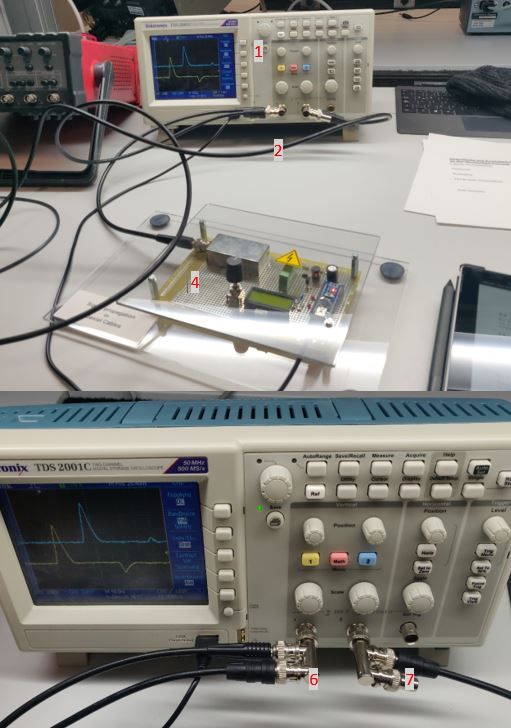
\includegraphics[width=.7\textwidth]{aufbau/setup_num.JPG}
        % \end{framed}
        %\includegraphics[width=12cm]{} % insert image (incl. numbering)
        \caption{Components needed for the experiment. 1. Oscilloscope, 2. Coaxial cables in various lengths, 3. Circuit board, 4. T-piece, \SI{50}{\ohm} transmission line terminator.}
        \label{fig:setup}
    \end{figure}
    %
    A detailed overview of the circuit board (position 3 in \cref{fig:setup}) will give \cref{fig:circuit_board} below.
    %
    \begin{figure}[H]
        \centering
        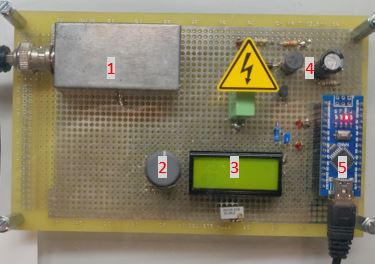
\includegraphics[width=.7\textwidth]{aufbau/circuit_board_num.JPG}
        \caption{Detailed view on the circuit board. 1. APG, 2. Potentiometer to adjust the voltage fed into the APG, 3. LC-Display to monitor
        the the BC's output voltage, 4. BC-circuit, 5. \micro-controller and PSU}
        \label{fig:circuit_board}
    \end{figure}
    %
\input{chapters/3_durchführung}
\chapter{Evaluation}
%
\section{Boost Converter}
    The characteristic curve of the BC is examined. In \cref{fig:characteristic-curve-of-the-boost-converter}
    the output voltage is plotted against the duty cycle. \textsc{SciDAVis} returns the linear fit of the measuring points as
    %
    \begin{figure}[h]
        \centering
        % 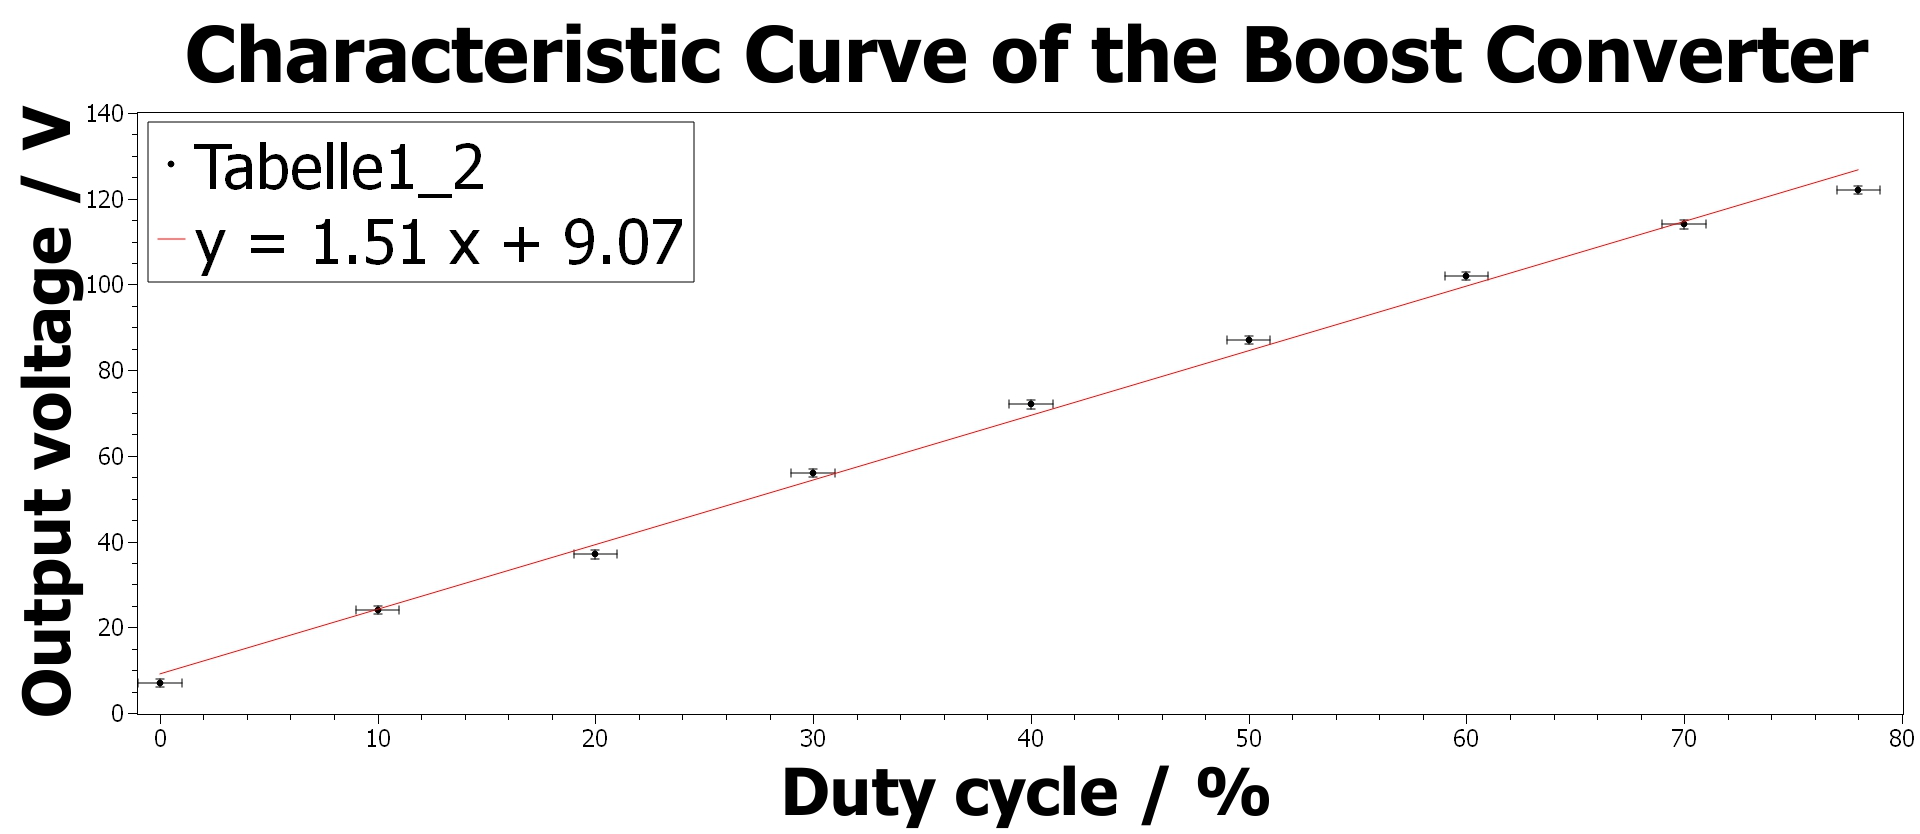
\includegraphics[width=\linewidth]{messdaten/Characteristic_Curve_of_the_Boost_Converter.jpg}
        \includesvg[inkscapelatex=false, width=.8\textwidth]{scidavis/Characteristic_Curve_of_the_Boost_Converter_mod}
        \caption[Characteristic curve of the BC]{Characteristic curve of the BC.}
        \label{fig:characteristic-curve-of-the-boost-converter}
    \end{figure}
    %
    \begin{equation}
        U_{out}(dc)=\frac{\SI{1.51}{V}}{\SI{1}{\percent}} \cdot dc + \SI{9.07}{V}
    \end{equation}
    %
    If the output voltages are compared with the simulated ones, there is observed a deviation of nearly \SI{10}{V} in the
    higher voltage area. The lower voltages, however, are similar.
    %
\section{Avalanche Pulse Generator}
    The signal in \cref{subfig:osci:avalanche_pulse_signal} is the first that appears after increasing the voltage to the minimum
    voltage $ U_{min}=\SI{70}{V} $. As discussed in \cref{sec:A3_charge-discharge-time} the time period at which the pulses
    occur and, thus, the repetition frequency is a function of the BC's output voltage \( U_+ \). Examining the
    actual behavior yields \cref{fig:repetition-frequency} (see \cref{subtab:3-1_duty_vs_voltage} for reference).
    %
    \begin{figure}[H]
        \centering
        % 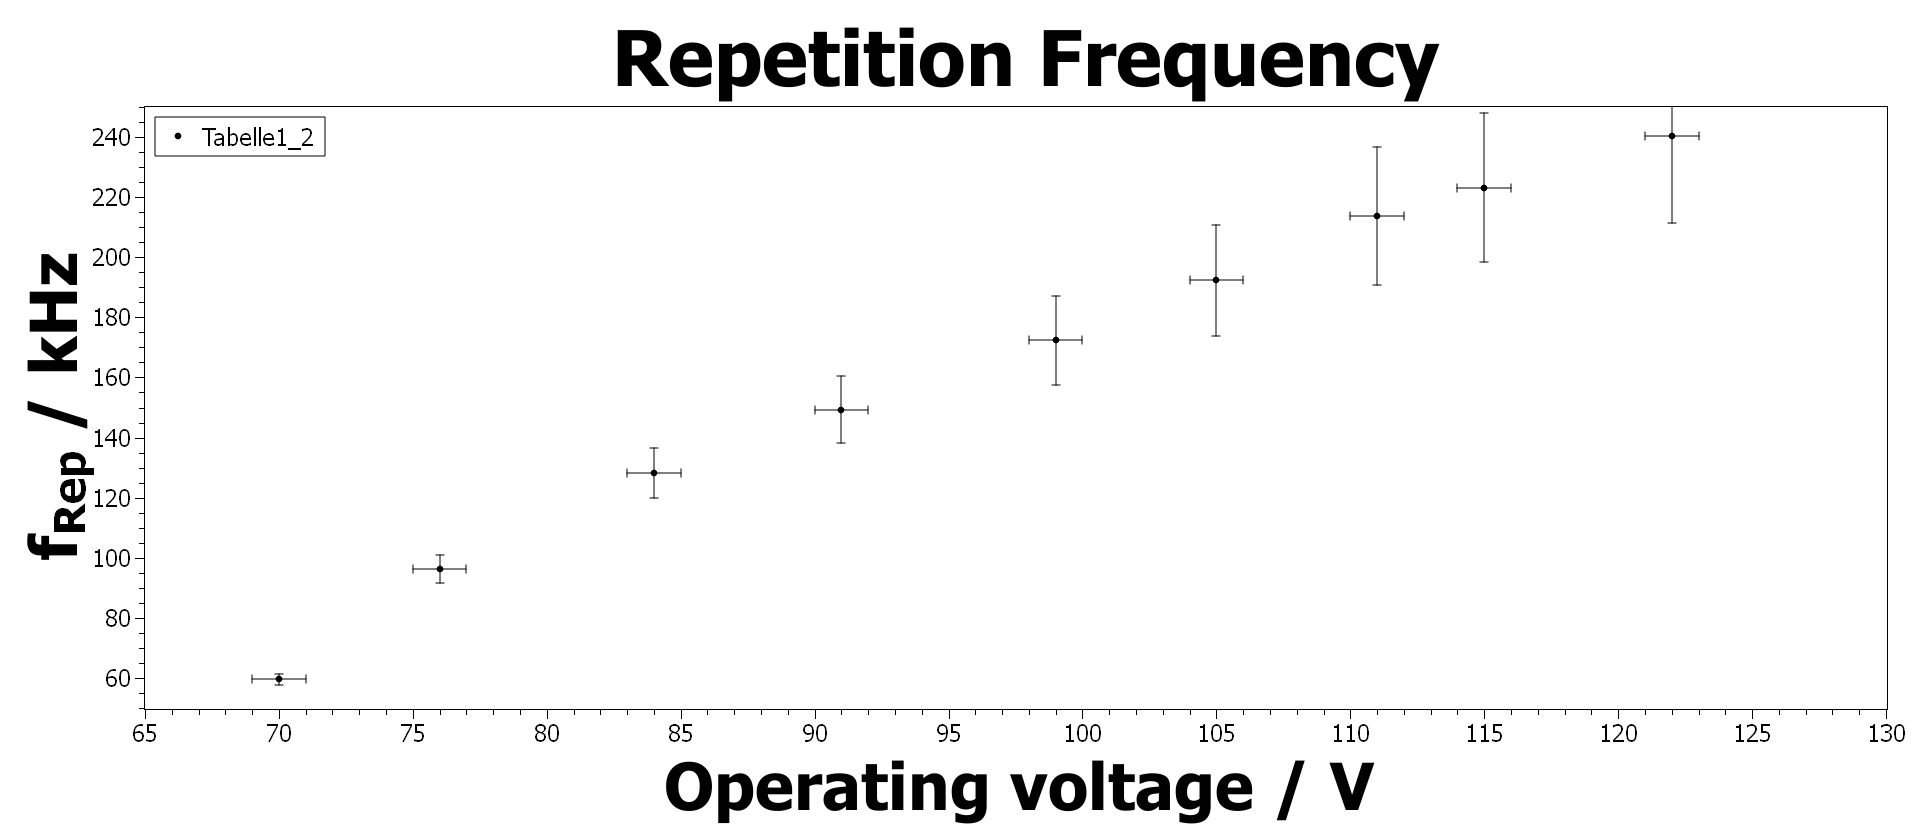
\includegraphics[width=1\linewidth]{messdaten/Repetition Frequency.jpg}
        \includesvg[inkscapelatex=false, width=.8\textwidth]{scidavis/repetition_frequency_mod}
        \caption[Examination repetition frequency over supply voltage]{Examination of the repetition frequency as a function of the supply voltage.}
        \label{fig:repetition-frequency}
    \end{figure}
    %
    The theoretical value for the repetition frequency at $ U=\SI{75}{V} $ with $ f_{Rep}=\SI{225.7}{kHz} $ (see \cref{sec:A3_charge-discharge-time})
    is larger by a factor. In the diagram in \cref{fig:repetition-frequency} the value is around
    $ \SI{90}{kHz} $. So there must be some deviations.\par\medskip
    Next the characteristics of the pulse at a voltage of $ U=\SI{75}{V} $ are examined. \Cref{subfig:osci:pulsuntersuchung}
    gives the following:
    %
    \begin{align}
        \text{Amplitude:}\qquad \hat{U}&=\SI{7.12}{V}\\
        \text{Rise time:}\qquad t_r&=\SI{2.33}{ns}\\
        \text{Fall time:}\qquad t_f&=\SI{7.08}{ns}\\
        \text{Pulse width:}\qquad t_w&=\SI{6.26}{ns}
    \end{align}
    %
    In comparison to a wave form captured with an oscilloscope of \SI{500}{MHz}, it can be seen that the secondary pulsations get suppressed
    quite significantly. Moreover, the signal features higher rise and fall time as well as having a lower amplitude.
    This is an expected behavior as discussed in \cref{sec:A5_oscopes_suitability}.
    %
    \begin{figure}[H]
        \centering
        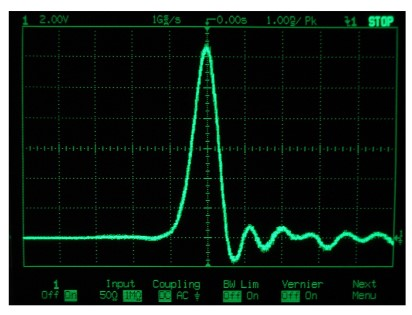
\includegraphics[width=.4\textwidth]{messdaten/500mhz_waveform.jpg}
        \caption[Pulse captured with a \SI{500}{MHz} oscilloscope]{A single pulse output by the APG and captured with an oscilloscope with \SI{500}{MHz}.}
        \label{fig:500MHz_waveform}
    \end{figure}
    %
\section{Signal Propagation}
%
    \subsection{Propagation Time}
        The propagation speed of a signal through a transmission line with known length is given by
        %
        \begin{equation}
            c_p=\frac{l}{t}
            \label{eq:propagation_speed}
        \end{equation}
        %
        The measured propagation times and the calculated propagation speeds are summarized in \cref{tab:delayed_signal}
        %
        \begin{table}[H]
            \caption{Delayed signal}
            \centering
            \begin{tabular}{@{}llll@{}}
                \toprule                                    
                Cable no.   & $ l \pm \Delta l $ \big/ \SI{}{m} & $ t \pm \Delta t $ \big/ \SI{}{ns}    & $ c_p \pm \Delta c_p $ \big/ \( \SI{}{\frac{m}{s}} \) \\ \midrule
                1           & $ 4.95 \pm 0.05 $                 & $ 22.6 \pm 1 $                        & $ (2.19\pm 0.12)\cdot 10^8 $ \\
                2           & $ 10.04 \pm 0.05 $                & $ 44.8 \pm 1 $                        & $ (2.24\pm 0.06)\cdot 10^8  $ \\
                3           & $ 0.77 \pm 0.01 $                 & $ 4.6 \pm 1 $                         & $ (1.67\pm 0.39)\cdot 10^8 $ \\ \bottomrule
            \end{tabular}
            \label{tab:delayed_signal}
        \end{table}
        %
        The error in propagation speed can be determined as follows:
        %
        \begin{align}
            \Delta c_p&=\left|\frac{\partial c_p}{\partial l}\right|\cdot \Delta l + \left|\frac{\partial c_p}{\partial t}\right|\cdot \Delta t \nonumber \\
            &=\frac{1}{t}\cdot \Delta l + \frac{l}{t^2} \cdot \Delta t
            \label{eq:cp_dev}
        \end{align}
        %
        For cable no. 1 in \cref{tab:delayed_signal} e.g.:
        %
        \begin{align}
            \Delta c_{P,1}&=\frac{1}{\SI{22.6}{\cdot 10^{-9}s}}\cdot \SI{0.05}{m} + \frac{\SI{4.95}{m}}{(\SI{22.6}{\cdot 10^{-9}s})^2} \cdot \SI{1}{\cdot 10^{-9}s} \nonumber \\
            &=\SI{0.02}{\cdot 10^8\frac{m}{s}}+\SI{0.10}{\cdot 10 ^8\frac{m}{s}} \nonumber \\
            &=\SI{0.12}{\cdot 10^8\frac{m}{s}}
        \end{align}
        %
    \subsection{Cable Characteristics}
        %
        \cref{subfig:osci:3-3-2_open_reflectionTime} shows the reflected pulse signal and \cref{subfig:osci:3-3-2_shorted} the shorted and reflected
        pulse signal.
        %
        The speed at which an electromagnetic signal propagates through a medium can be calculated by
        \begin{equation}
            c_p = \left(\sqrt{\varepsilon_0\varepsilon_r}\right)^{-1} \left(\sqrt{\mu_0\mu_r}\right)^{-1}
        \end{equation}
        where \( \left(\sqrt{\varepsilon_0\mu_0}\right)^{-1} \) is the speed of light. Sent through a medium other than
        vacuum the electric and magnetic properties of the medium reduce the propagation speed by a factor of \( \left(\sqrt{\varepsilon_r\mu_r}\right)^{-1} \) \cite{Halliday.2005}.
        A metric to quantify the relative speed of propagation is the velocity factor:
        \begin{equation}
            VF = \frac{c_p}{c_0}
        \end{equation}
        At the minimum amplitude of the reflected pulse, the resistance \( R_{Term} \) equals \( Z_0 \).\par
        The determined and calculated characteristic values are summarized in the following table:
        %
        \begin{table}[h]
            \caption{Reflected signal}
            \begin{adjustbox}{width=\textwidth,keepaspectratio}
                \begin{tabular}{@{}llllllll@{}}
                    \toprule
                    Cable no.   & $ l $ \big/ \SI{}{m}  & $ \tau_0 $ \big/ \SI{}{ns}    & $ \tau_s $ \big/ \SI{}{ns}    & $ c_p $ \big/ $ \SI{}{\frac{m}{s}} $  & $ VF $ \big/ \%   & $ Z_0 $ \big/ $\Omega$    & $\varepsilon_R$ \\ \midrule
                    1           & $ 4.95 \pm 0.05 $     & $ 44.8 \pm 1 $                & $ 44.8 \pm 1 $                & $ (2.21\pm 0.07)\cdot 10^8 $          & $ 73.7 \pm 2.3 $  & 80.2                      & $ 1.84 \pm 0.11 $ \\
                    2           & $ 10.04 \pm 0.05 $    & $ 89.6 \pm 1 $                & $ 90.4 \pm 1 $                & $ (2.24\pm 0.04)\cdot 10^8 $          & $ 74.7 \pm 1.3 $  & 56.0                      & $ 1.79 \pm 0.06 $ \\
                    3           & $ 0.77 \pm 0.01 $     & $ 8.4 \pm 1 $                 & $ 10.8 \pm 1 $                & $ (1.83\pm 0.34)\cdot 10^8 $          & $ 61.0 \pm 11.3 $ & 56.4                      & $ 2.69 \pm 1.00 $ \\ \bottomrule
                \end{tabular}
            \end{adjustbox}
            \label{tab:reflected_signal}
        \end{table}
        %
        The deviation of $ c_p $ can be determined similar to \cref{eq:cp_dev}, but with a factor of 2. The delta in $ VF $ as follows:
        %
        \begin{align}
            \Delta VF&=\left|\frac{\partial VF}{\partial c_p}\right|\cdot \Delta c_p \nonumber \\
            &=\frac{1}{c_0}\cdot \Delta c_p
        \end{align}
        %
        For cable no. 1 in \cref{tab:reflected_signal} e.g.:
        %
        \begin{equation}
            \Delta VF_1=\frac{1}{\SI{3}{\cdot 10^8 \frac{m}{s}}}\cdot \SI{0.07}{\frac{m}{s}}=2.3\%
        \end{equation}
        %
        And for $ \varepsilon_R $:
        %
        \begin{equation}
            \Delta \varepsilon_R = \left|\frac{\partial \varepsilon_R}{\partial VF}\right|\cdot \Delta VF = \frac{2}{VF^3} \cdot \Delta VF
        \end{equation}
        %
        So for the first cable in \cref{tab:reflected_signal}:
        %
        \begin{equation}
            \Delta \varepsilon_{R,1}=\frac{2}{0.737^3}\cdot 0.023=0.11
        \end{equation}
        %
        If the values are compared with the data sheet from the manufacturer, there can be seen some similarities and differences.
        The determined velocity factor of cable no. 1 and 2 is very close to the stated one (69.5\%). The third cable is slightly
        different.\par
        On the other hand, the impedance is given as $ \SI{53}{\Omega} $, with the second and third cable having a similar value,
        whereas the first cable differs somewhat.
        %
    \subsection{Time Domain Reflectometry}
        For determining the unknown length and the position of the fault of the cable, the equation for the propagation speed has
        to be transformed to the length as
        %
        \begin{equation}
            l=\frac{1}{2}\cdot c_p \cdot \tau
            \label{eq:length}
        \end{equation}
        %
        $\tau_{total}$ has been measured as \SI{276}{ns} and $\tau_{fault}$ as \SI{256}{ns}.
        For the propagation speed the mean value $ \bar{c_p} = \SI{2.09 \cdot 10^8}{\frac{m}{s}} $ is used. The values inserted in
        \cref{eq:length} results:
        %
        \begin{align*}
            l_{total}&=\frac{1}{2}\cdot\SI{2.09}{\cdot 10^8\frac{m}{s}}\cdot \SI{276}{\cdot 10^{-9} s}=\SI{28.84}{m}\\
            l_{fault}&=\frac{1}{2}\cdot\SI{2.09}{\cdot 10^8\frac{m}{s}}\cdot \SI{256}{\cdot 10^{-9} s}=\SI{26.75}{m}
        \end{align*}
        %
        The deviation is determined with the following equation:
        %
        \begin{align}
            \Delta l&=\left|\frac{\partial l}{\partial c_p}\right|\cdot \Delta c_p + \left|\frac{\partial l}{\partial \tau}\right|\cdot \Delta \tau\\
            &=\frac{1}{2}\cdot \tau \cdot \Delta c_p + \frac{1}{2}\cdot c_p \cdot \Delta \tau
        \end{align}
        %
        For the total length and the position of the defect:
        \begin{align*}
            \Delta l_{total}&=\frac{1}{2} \cdot\SI{276}{\cdot 10^{-9}s}\cdot \SI{0.15}{\cdot 10^8\frac{m}{s}}  + \frac{1}{2}\cdot \SI{2.09}{\cdot 10^8\frac{m}{s}} \cdot\SI{1}{\cdot 10^{-9}s}\\
            &=\SI{2.07}{m}+\SI{0.10}{m}\\
            &=\SI{2.17}{m}\\
            \\
            \Delta l_{fault}&=\SI{2.02}{m}
        \end{align*}
        %
        Summarized the total length is
        %
        \begin{equation}
            l_{total}=\SI{28.8}{m} \pm \SI{2.2}{m}
        \end{equation}
        %
        and the position of the fault is at
        %
        \begin{equation}
            l_{fault}=\SI{26.8}{m} \pm \SI{2.0}{m}
        \end{equation}
\chapter{Conclusion}
%
Muss noch erstellt werden

fehlt noch bisschen was

"bisschen" 
%-------------------
\newpage
\listoffigures 
\listoftables
\addchap{List of Symbols}
\begin{table}[h]
    \begin{tabular}{@{}ll@{}}%
        \( B \) & Bandwidth\\
        \( C \) & Capacitor\\
        \( c_p \) & Propagation speed\\
        \( c_0 \) & Speed of light\\
        \( dc \) & PWM duty cycle \\
		\( f_{Rep} \) & Repetition frequency\\
		\( l \) & Cable length\\
		\( l_{fault} \) & Length to defect\\
        \( l_{total} \) & Total length of cable\\
        \( R \) & Resistor\\
		\( R_{Term} \) & Impedance matching the characteristic impedance\\
        \( t \) & Time\\
        \( t_{10\%} \) & Time to 10\% of the amplitude\\
        \( t_{90\%} \) & Time to 90\% of the amplitude\\
		\( t_{chrg} \) & Charging time\\
		\( t_{dchrg} \) & Discharging time\\
		\( t_f \) & Fall time\\
		\( t_w \) & Pulse width\\
		\( t_{r} \) & Rise time\\
		\( \hat{U} \) & Amplitude\\
        \( U_{Br} \) & Threshold voltage\\
        \( U_C \) & Voltage across a capacitor \\
		\( U_{min} \) & Minimum operating voltage\\
		\( U_{+} \) & Output voltage\\
		\( VF \) & Velocity factor\\
        \( Z_0 \) & Characteristic impedance\\
        & \\
        \( \Delta c_p \) & \\
        \( \Delta l \) & \\
        \( \Delta l_{fault} \) & \\
        \( \Delta l_{total} \) & \\
        \( \Delta t \) & \\
        \( \Delta VF \) & \\
        \( \Delta \tau \) & \\
        \( \mu_0 \) & \\
        \( \mu_r \) & \\
		\( \tau_0 \) & Propagation time with open end\\
		\( \tau_{fault} \) & Propagation time to the defective point\\
		\( \tau_s \) & Propagation time with short-circuited end\\
        \( \tau_{total} \) & Propagation time for the full length\\
        \( \varepsilon_0 \) & \\
		\( \varepsilon_r \) & Relative permittivity\\
    \end{tabular}
    \label{tab:glossar}
\end{table}
\appendix
\chapter{Appendix}
%
\begin{figure}[h]%
    \centering
    \subfloat[Reference pulse at CH1. The delayed pulse is fed to CH2.\label{subfig:osci:ch1-ch2_delayed_pulse}]
    {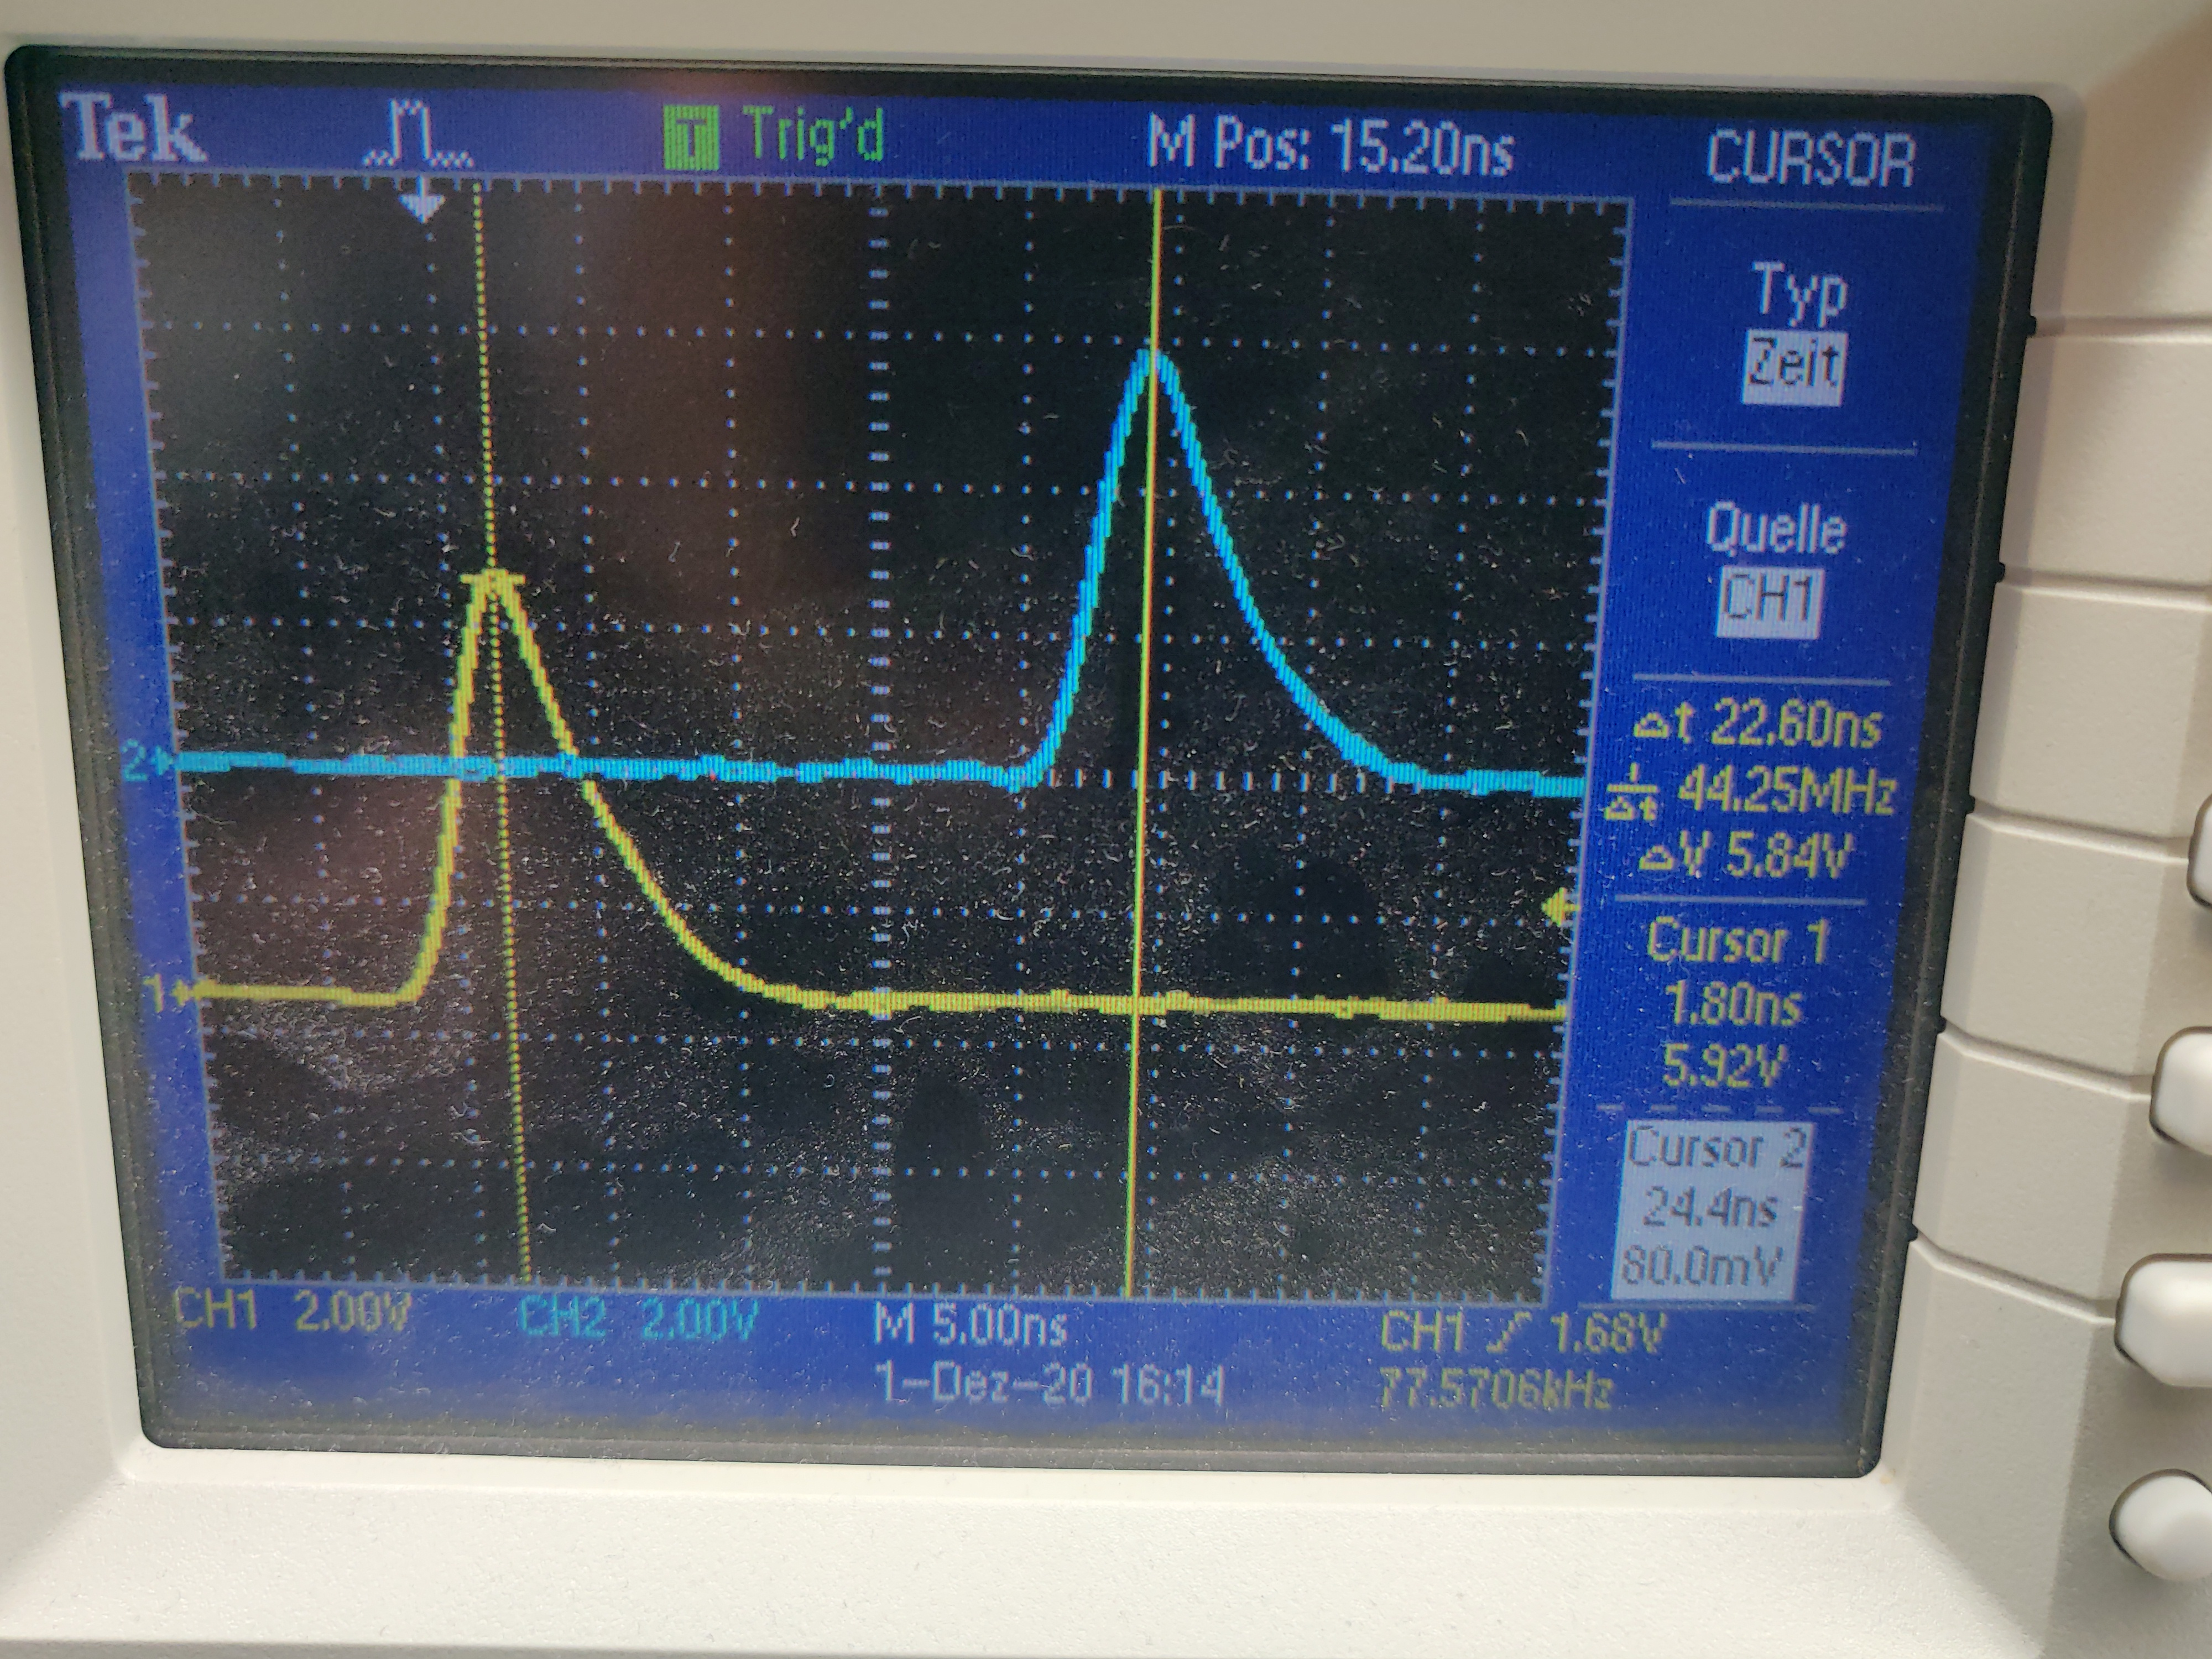
\includegraphics[width=0.45\linewidth]{messdaten/3-3-1_propagationDelay.jpg}}%
    \hspace{.05\linewidth}
    \subfloat[The reference pulse gets reflected at an open-ended cable connected to the same channel. A difference in time due to a finite propagation speed can be observed.\label{subfig:osci:3-3-2_open_reflectionTime}]
    {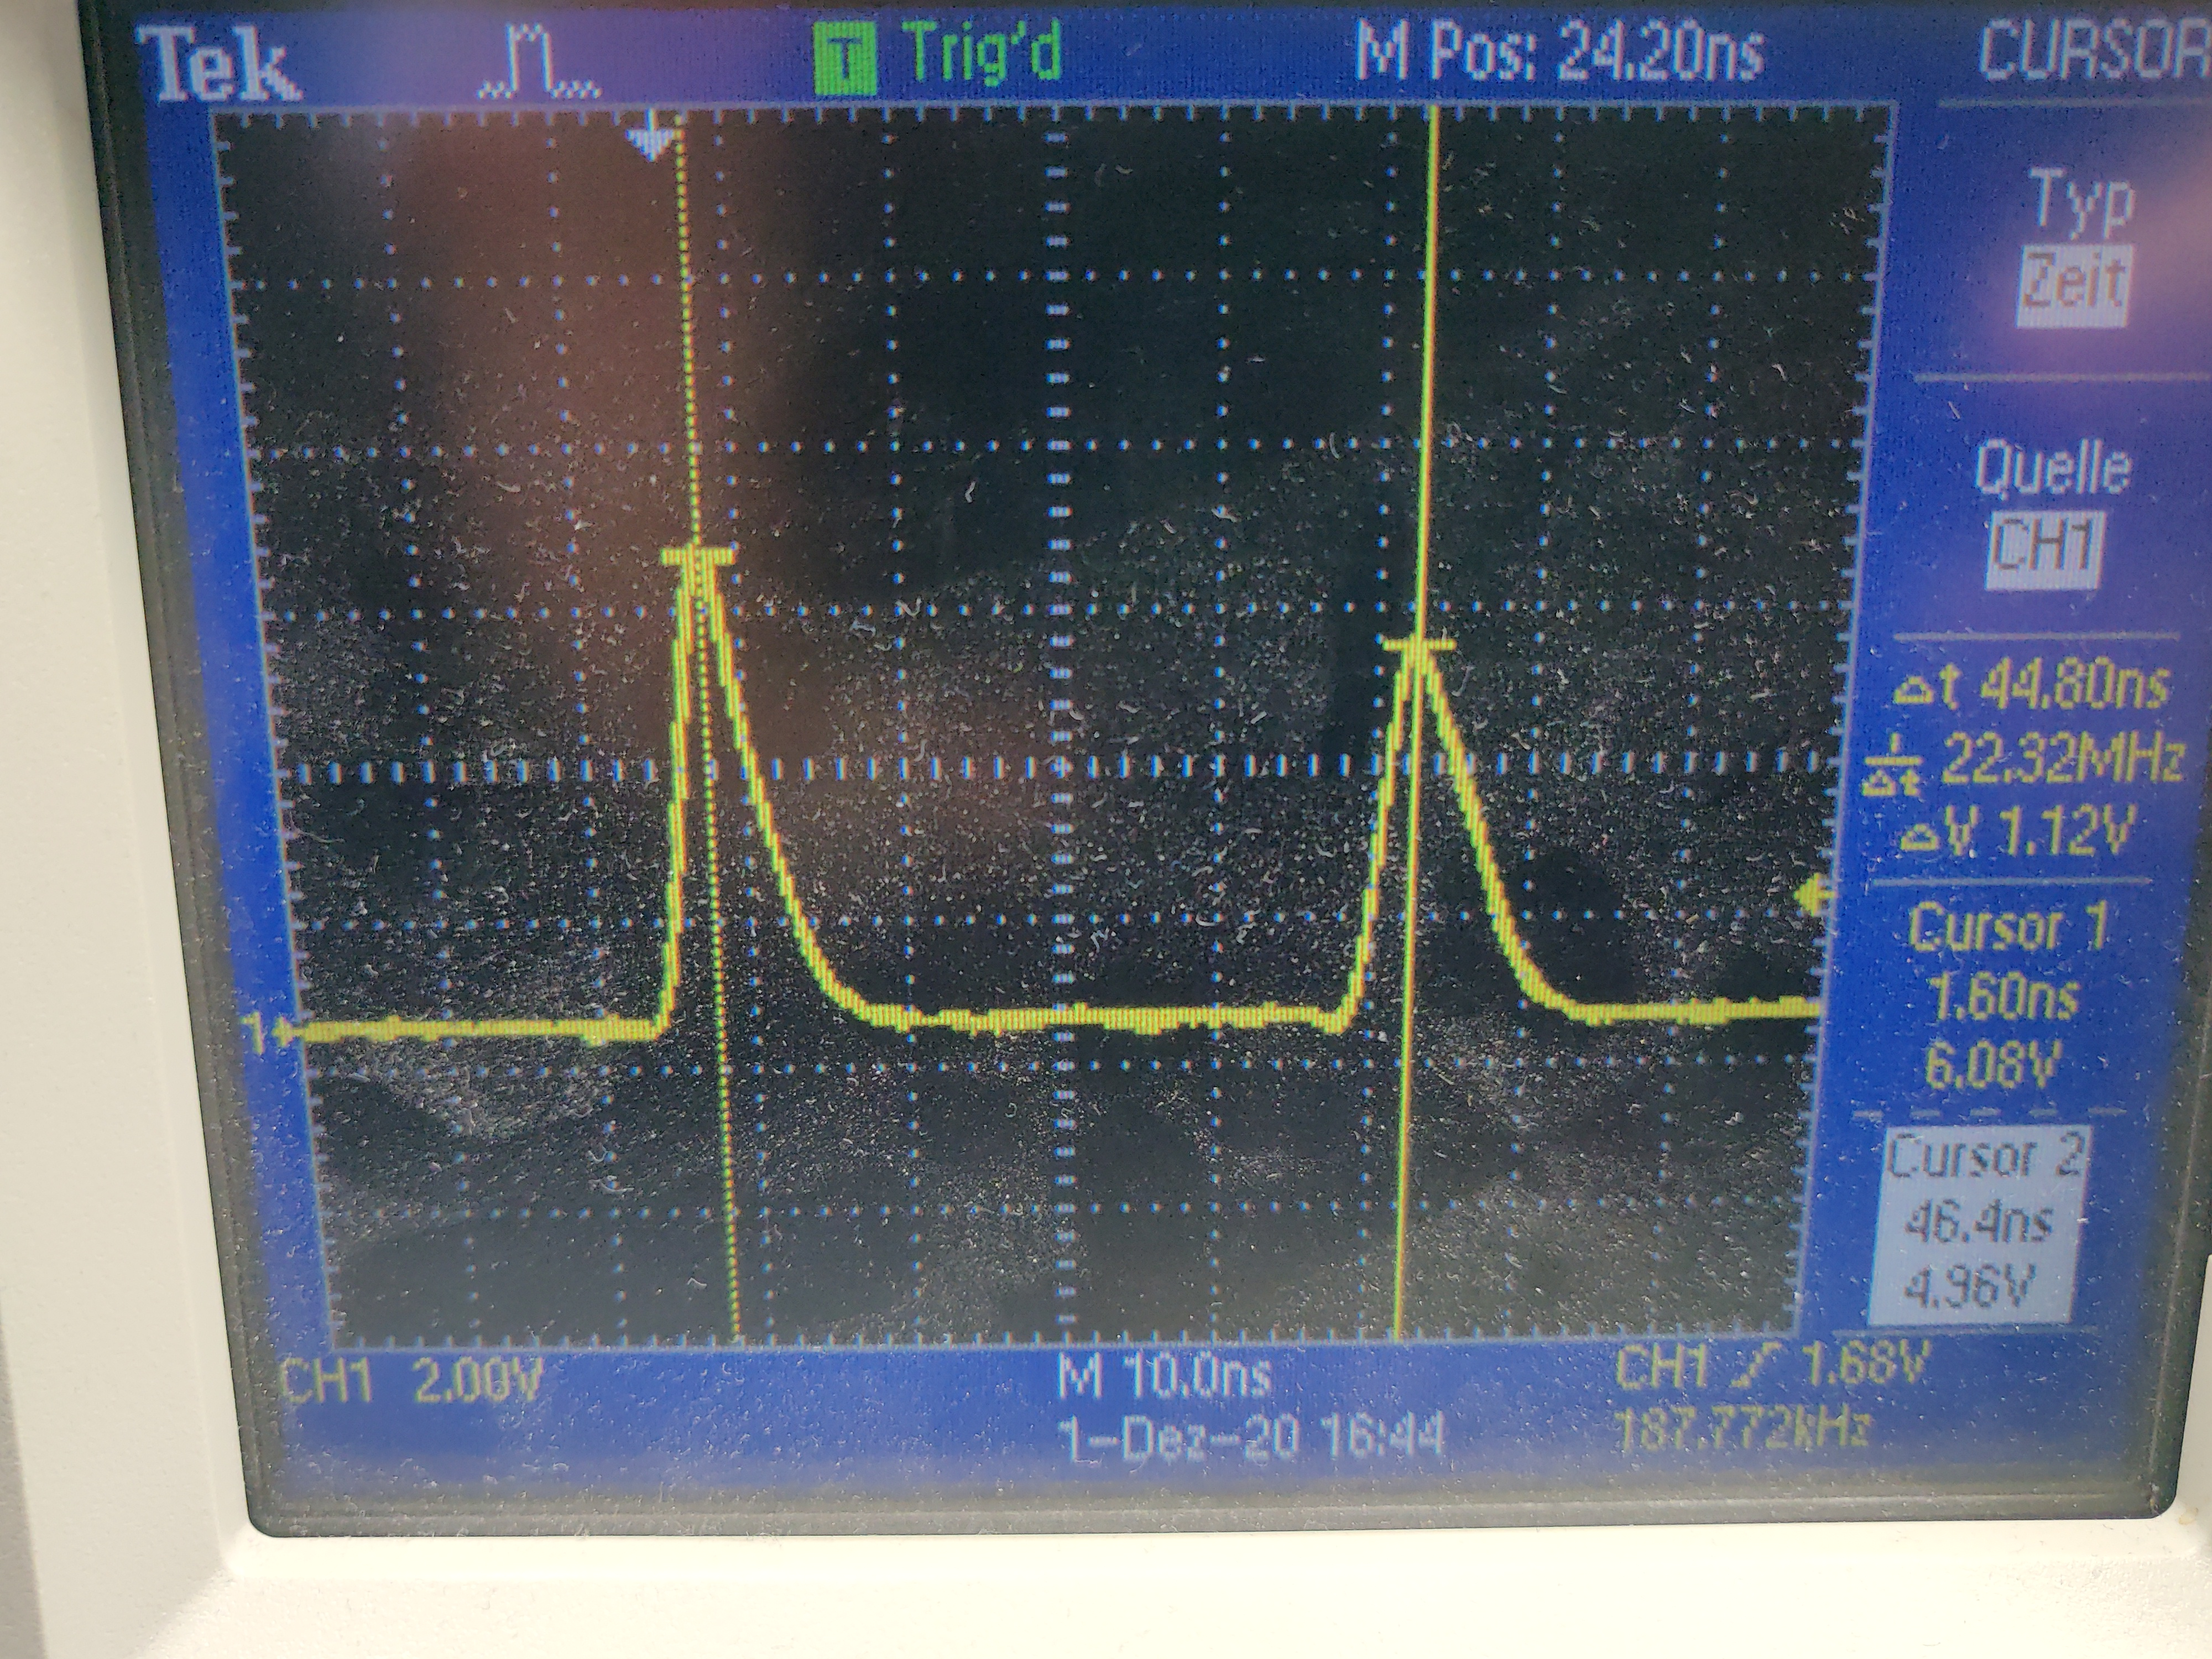
\includegraphics[width=0.45\linewidth]{messdaten/3-3-2_open_reflectionTime.jpg}}\\%
    \subfloat[If the transmission line gets terminated with an impedance close to zero, the reflected pulse gets inverted.\label{subfig:osci:3-3-2_shorted}]
    {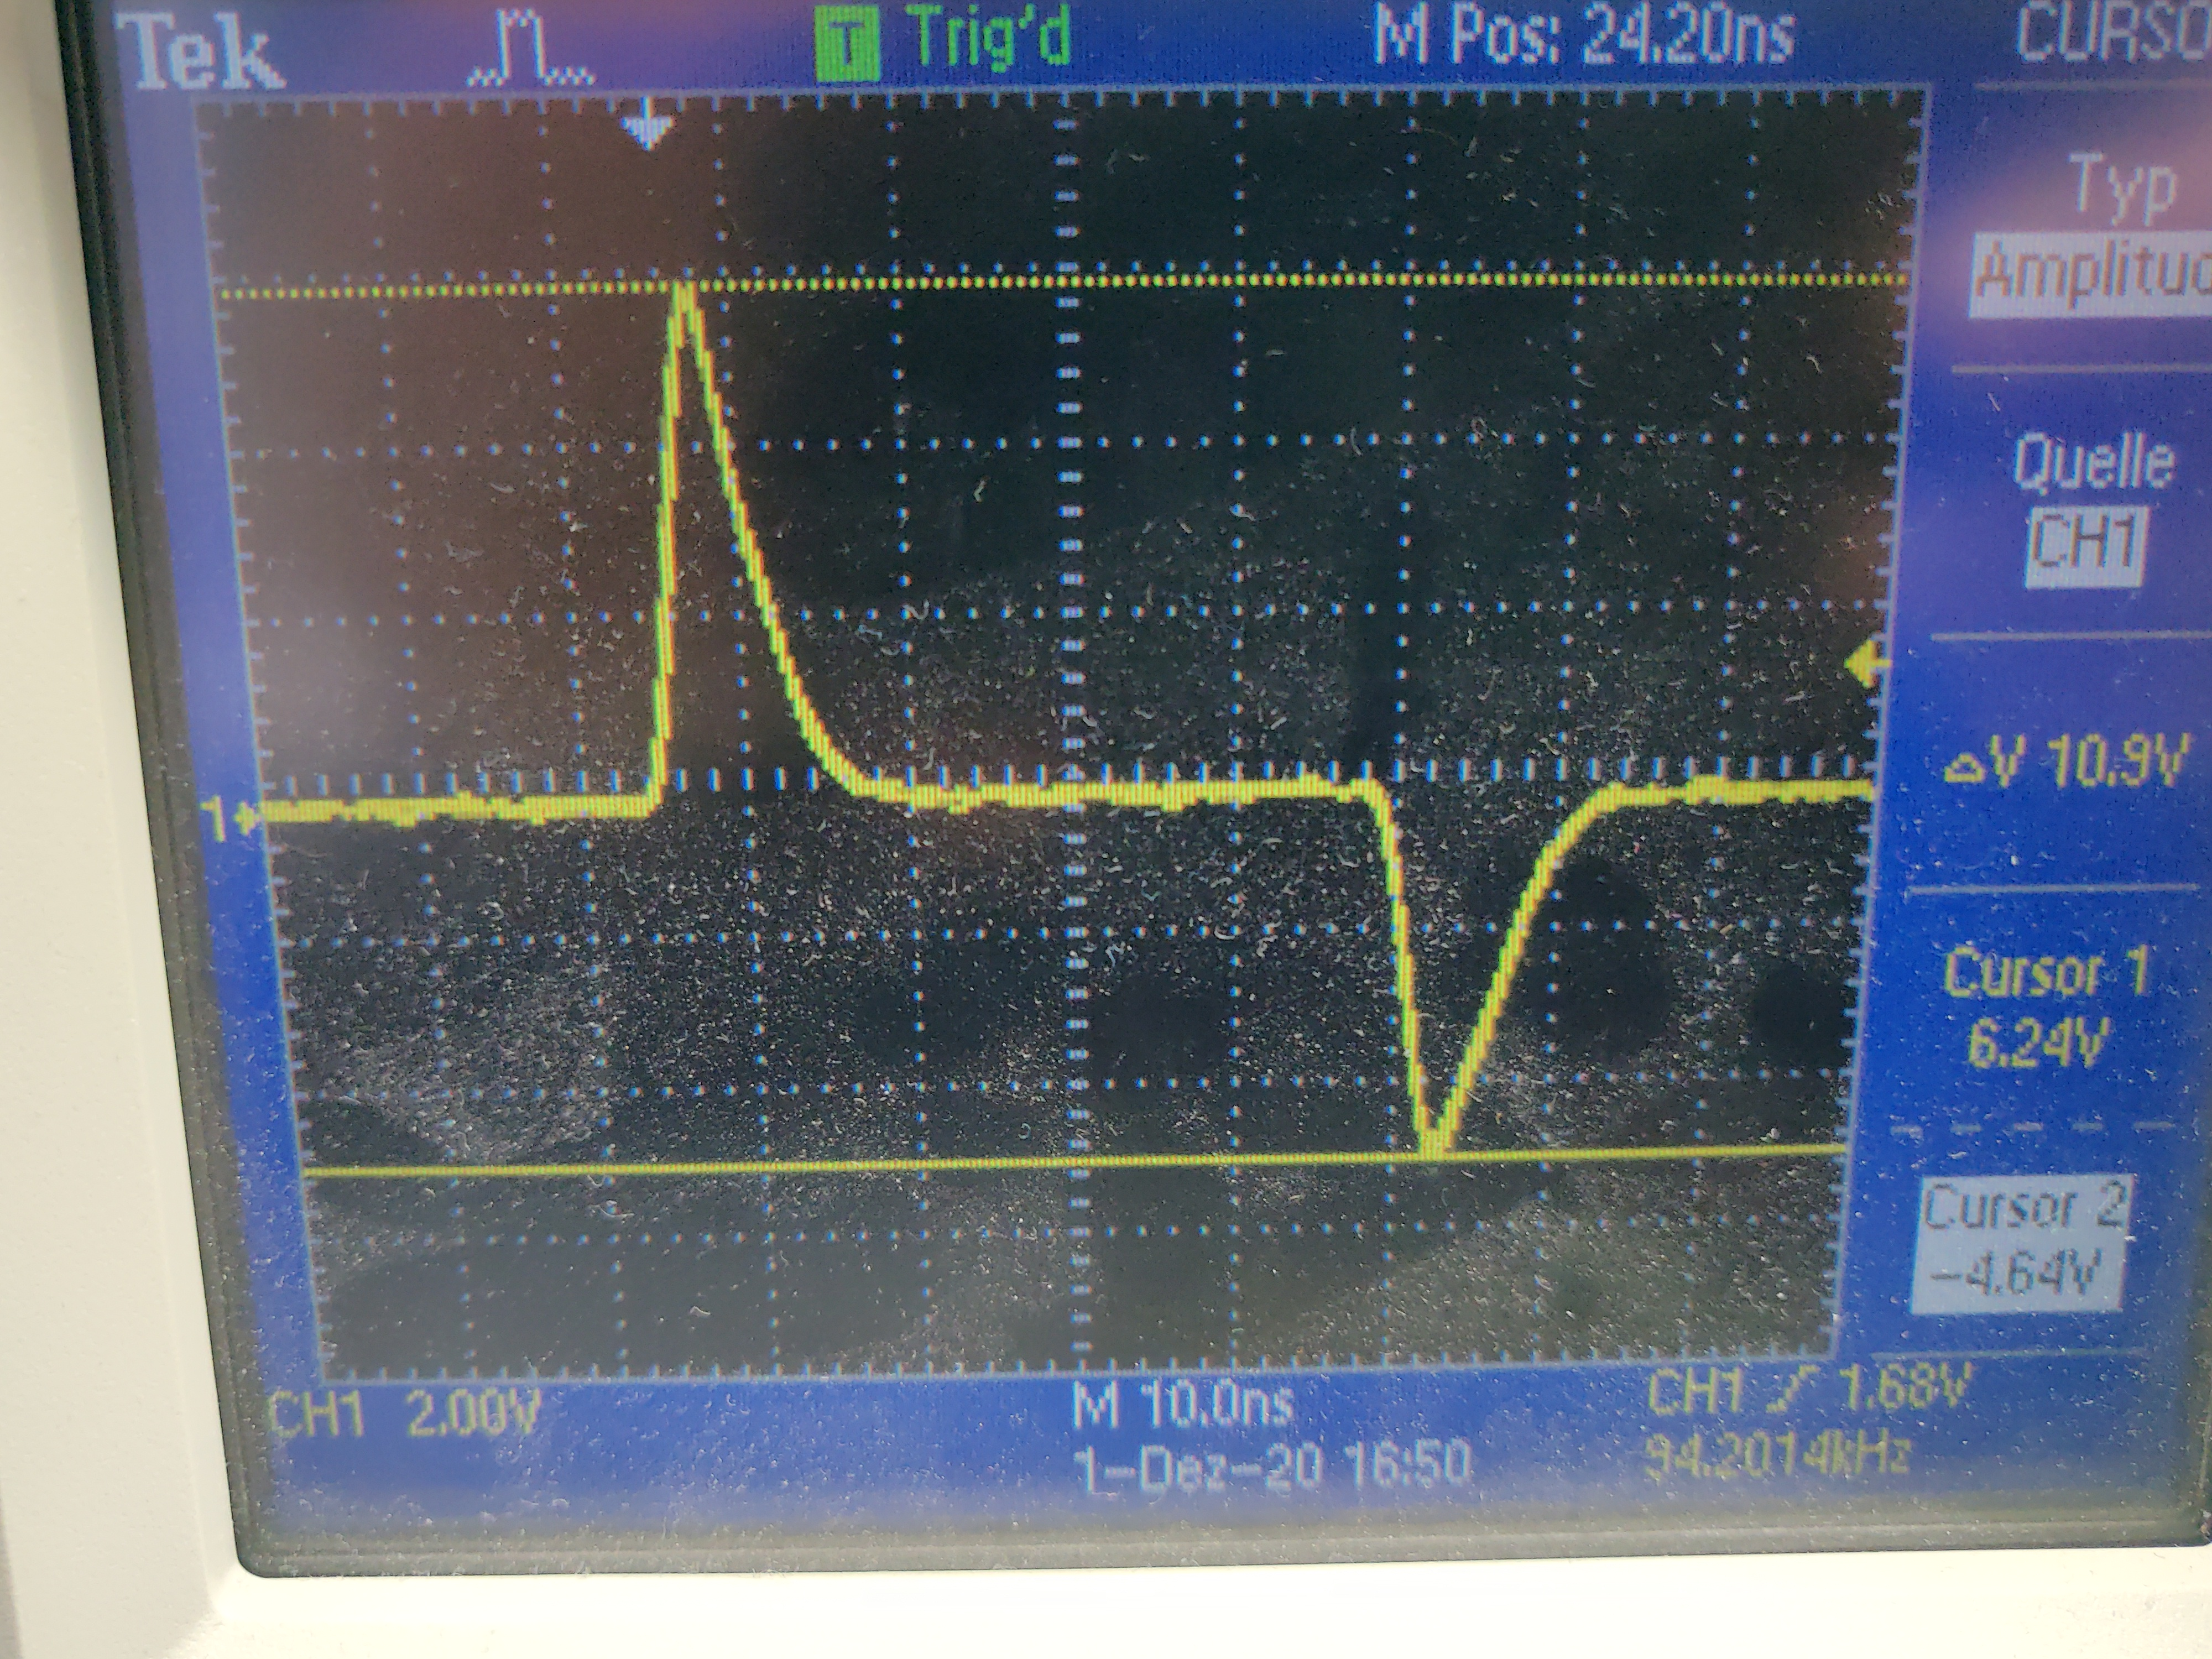
\includegraphics[width=0.45\linewidth]{messdaten/3-3-2_shorted.jpg}}%
    \hspace{.05\linewidth}
    \subfloat[The reflected signal can almost completely inhibited terminating the transmission line with an impedance close to its characteristic impedance.\label{subfig:osci:3-3-2_Z_0_equal_R_term}]
    {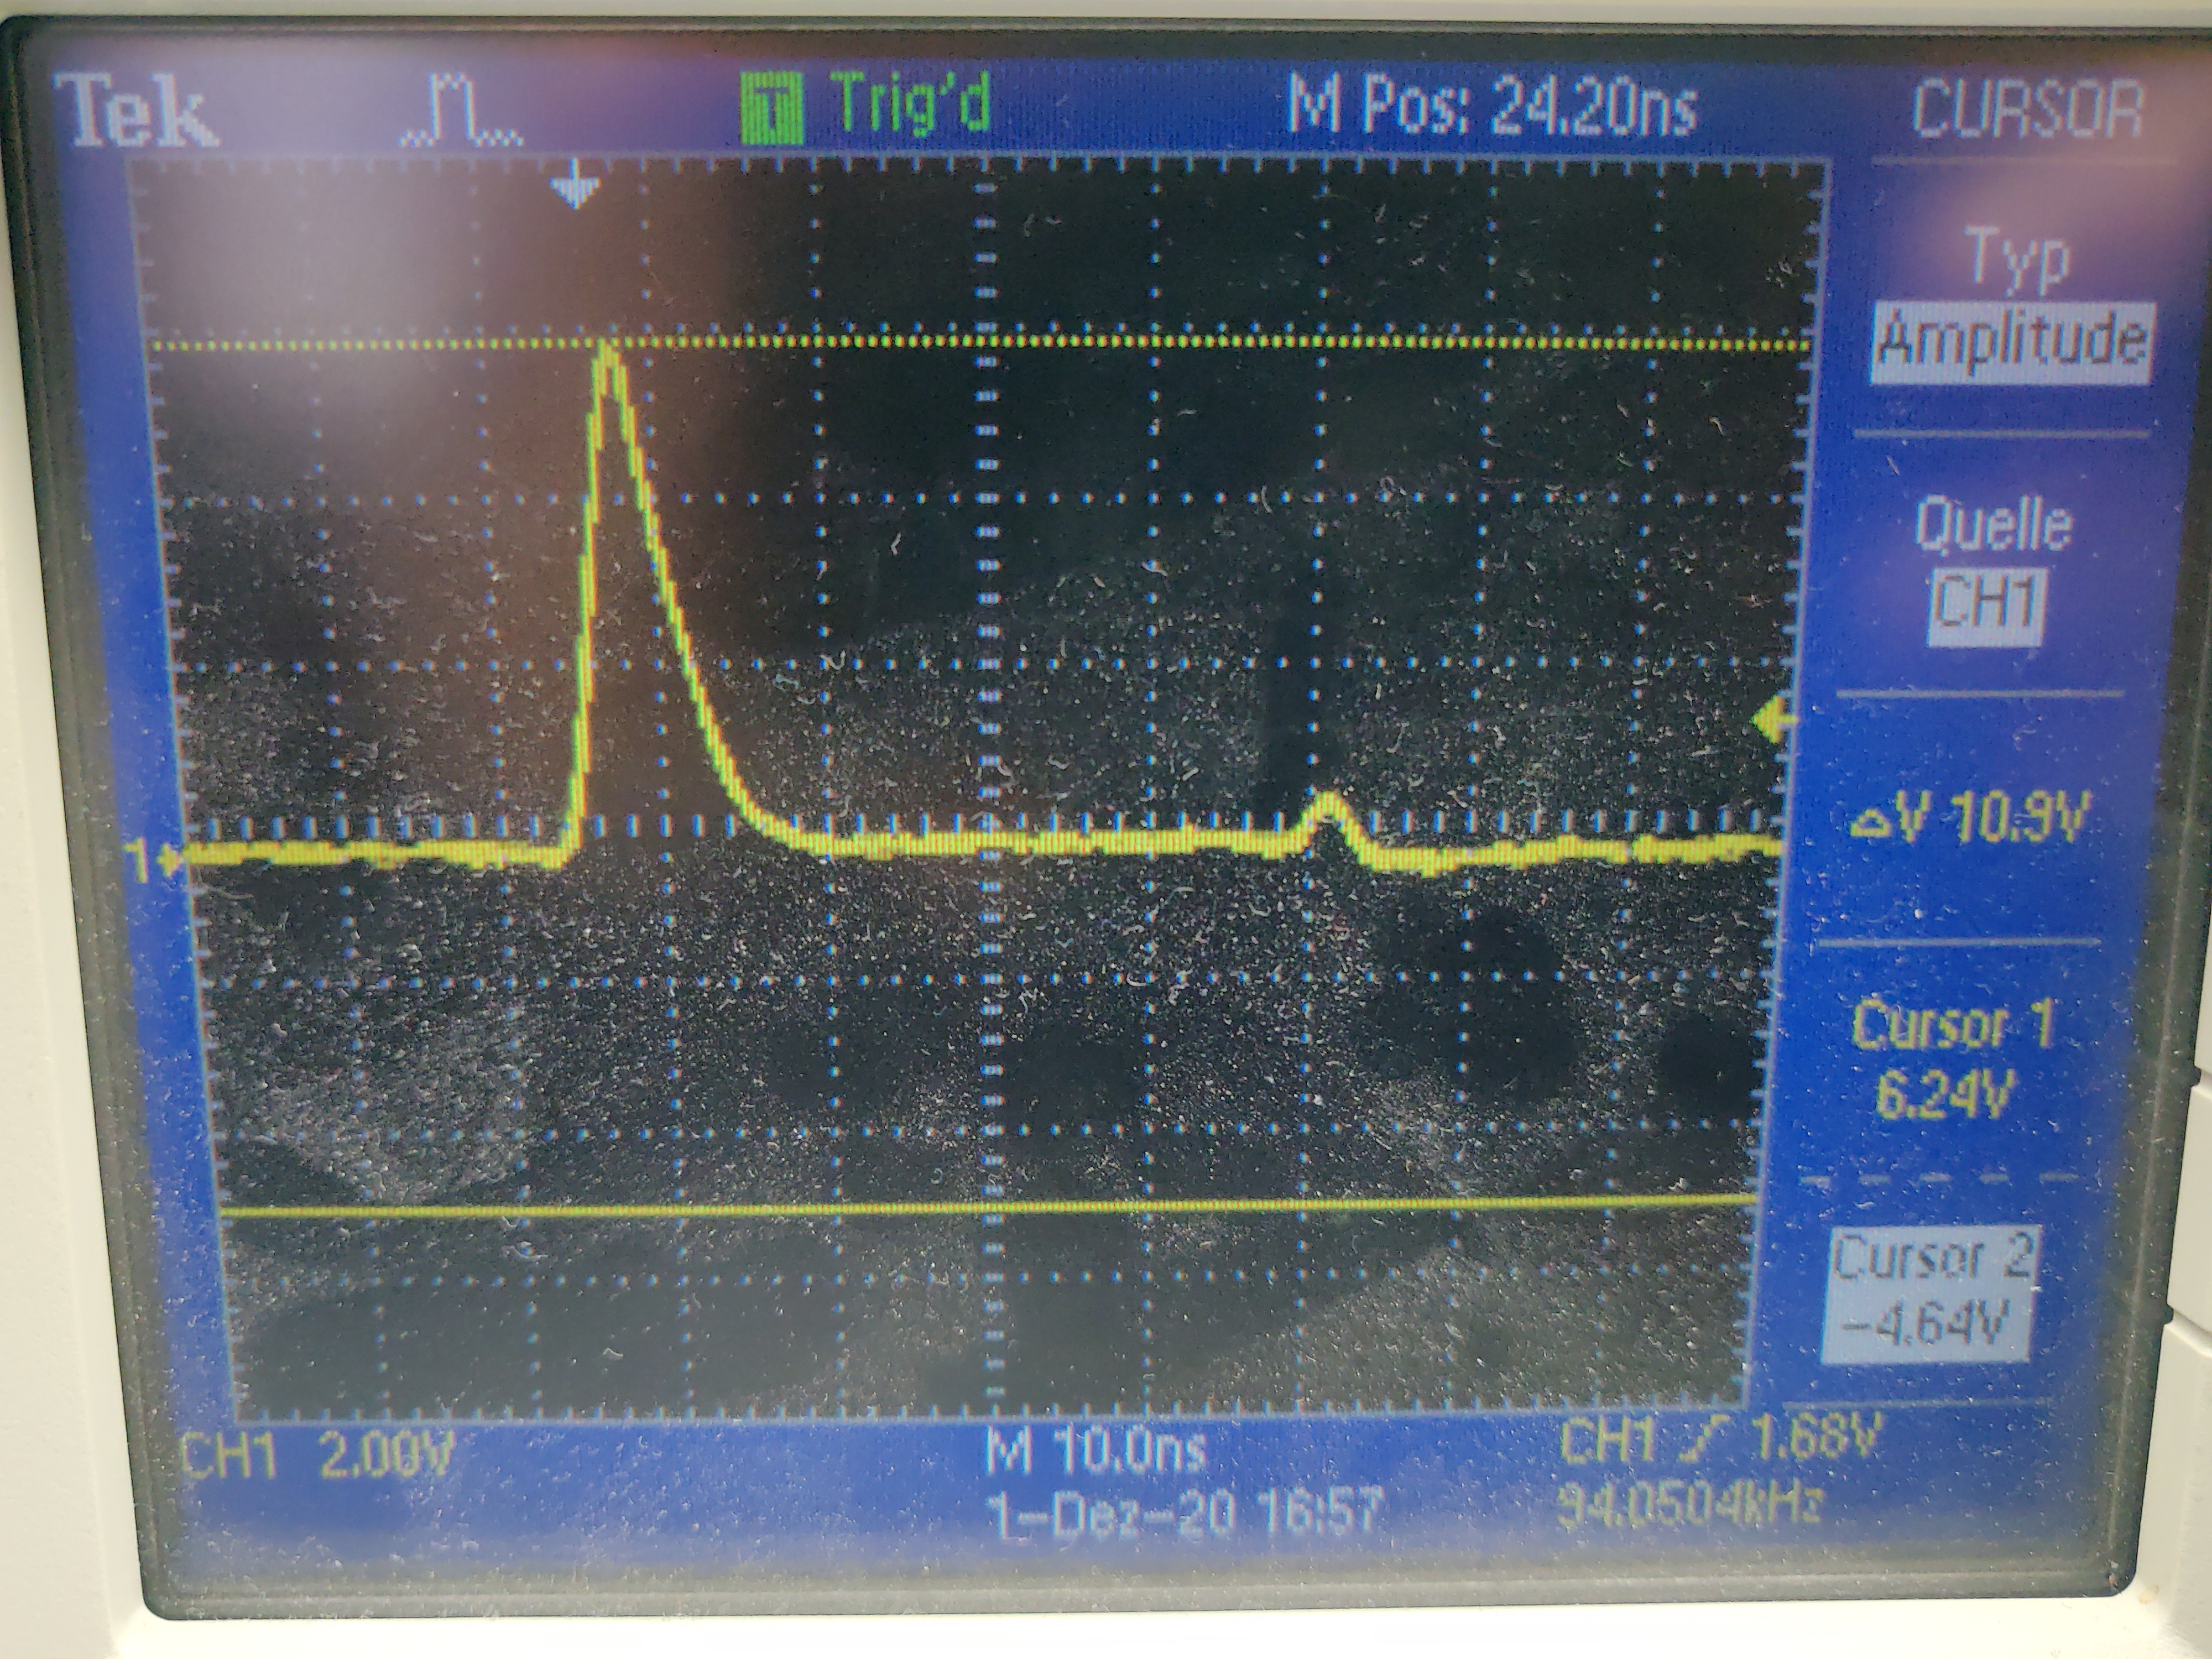
\includegraphics[width=0.45\linewidth]{messdaten/3-3-2_Z_0_equal_R_term.jpg}}%
\end{figure}
\begin{figure}[h]
    \ContinuedFloat%
    \subfloat[Local changes to the cables characteristics reflect signals as well. This can be utilized to locate a defect along the cable's length.\label{subfig:osci:3-3-3_lengthToDefect}]
    {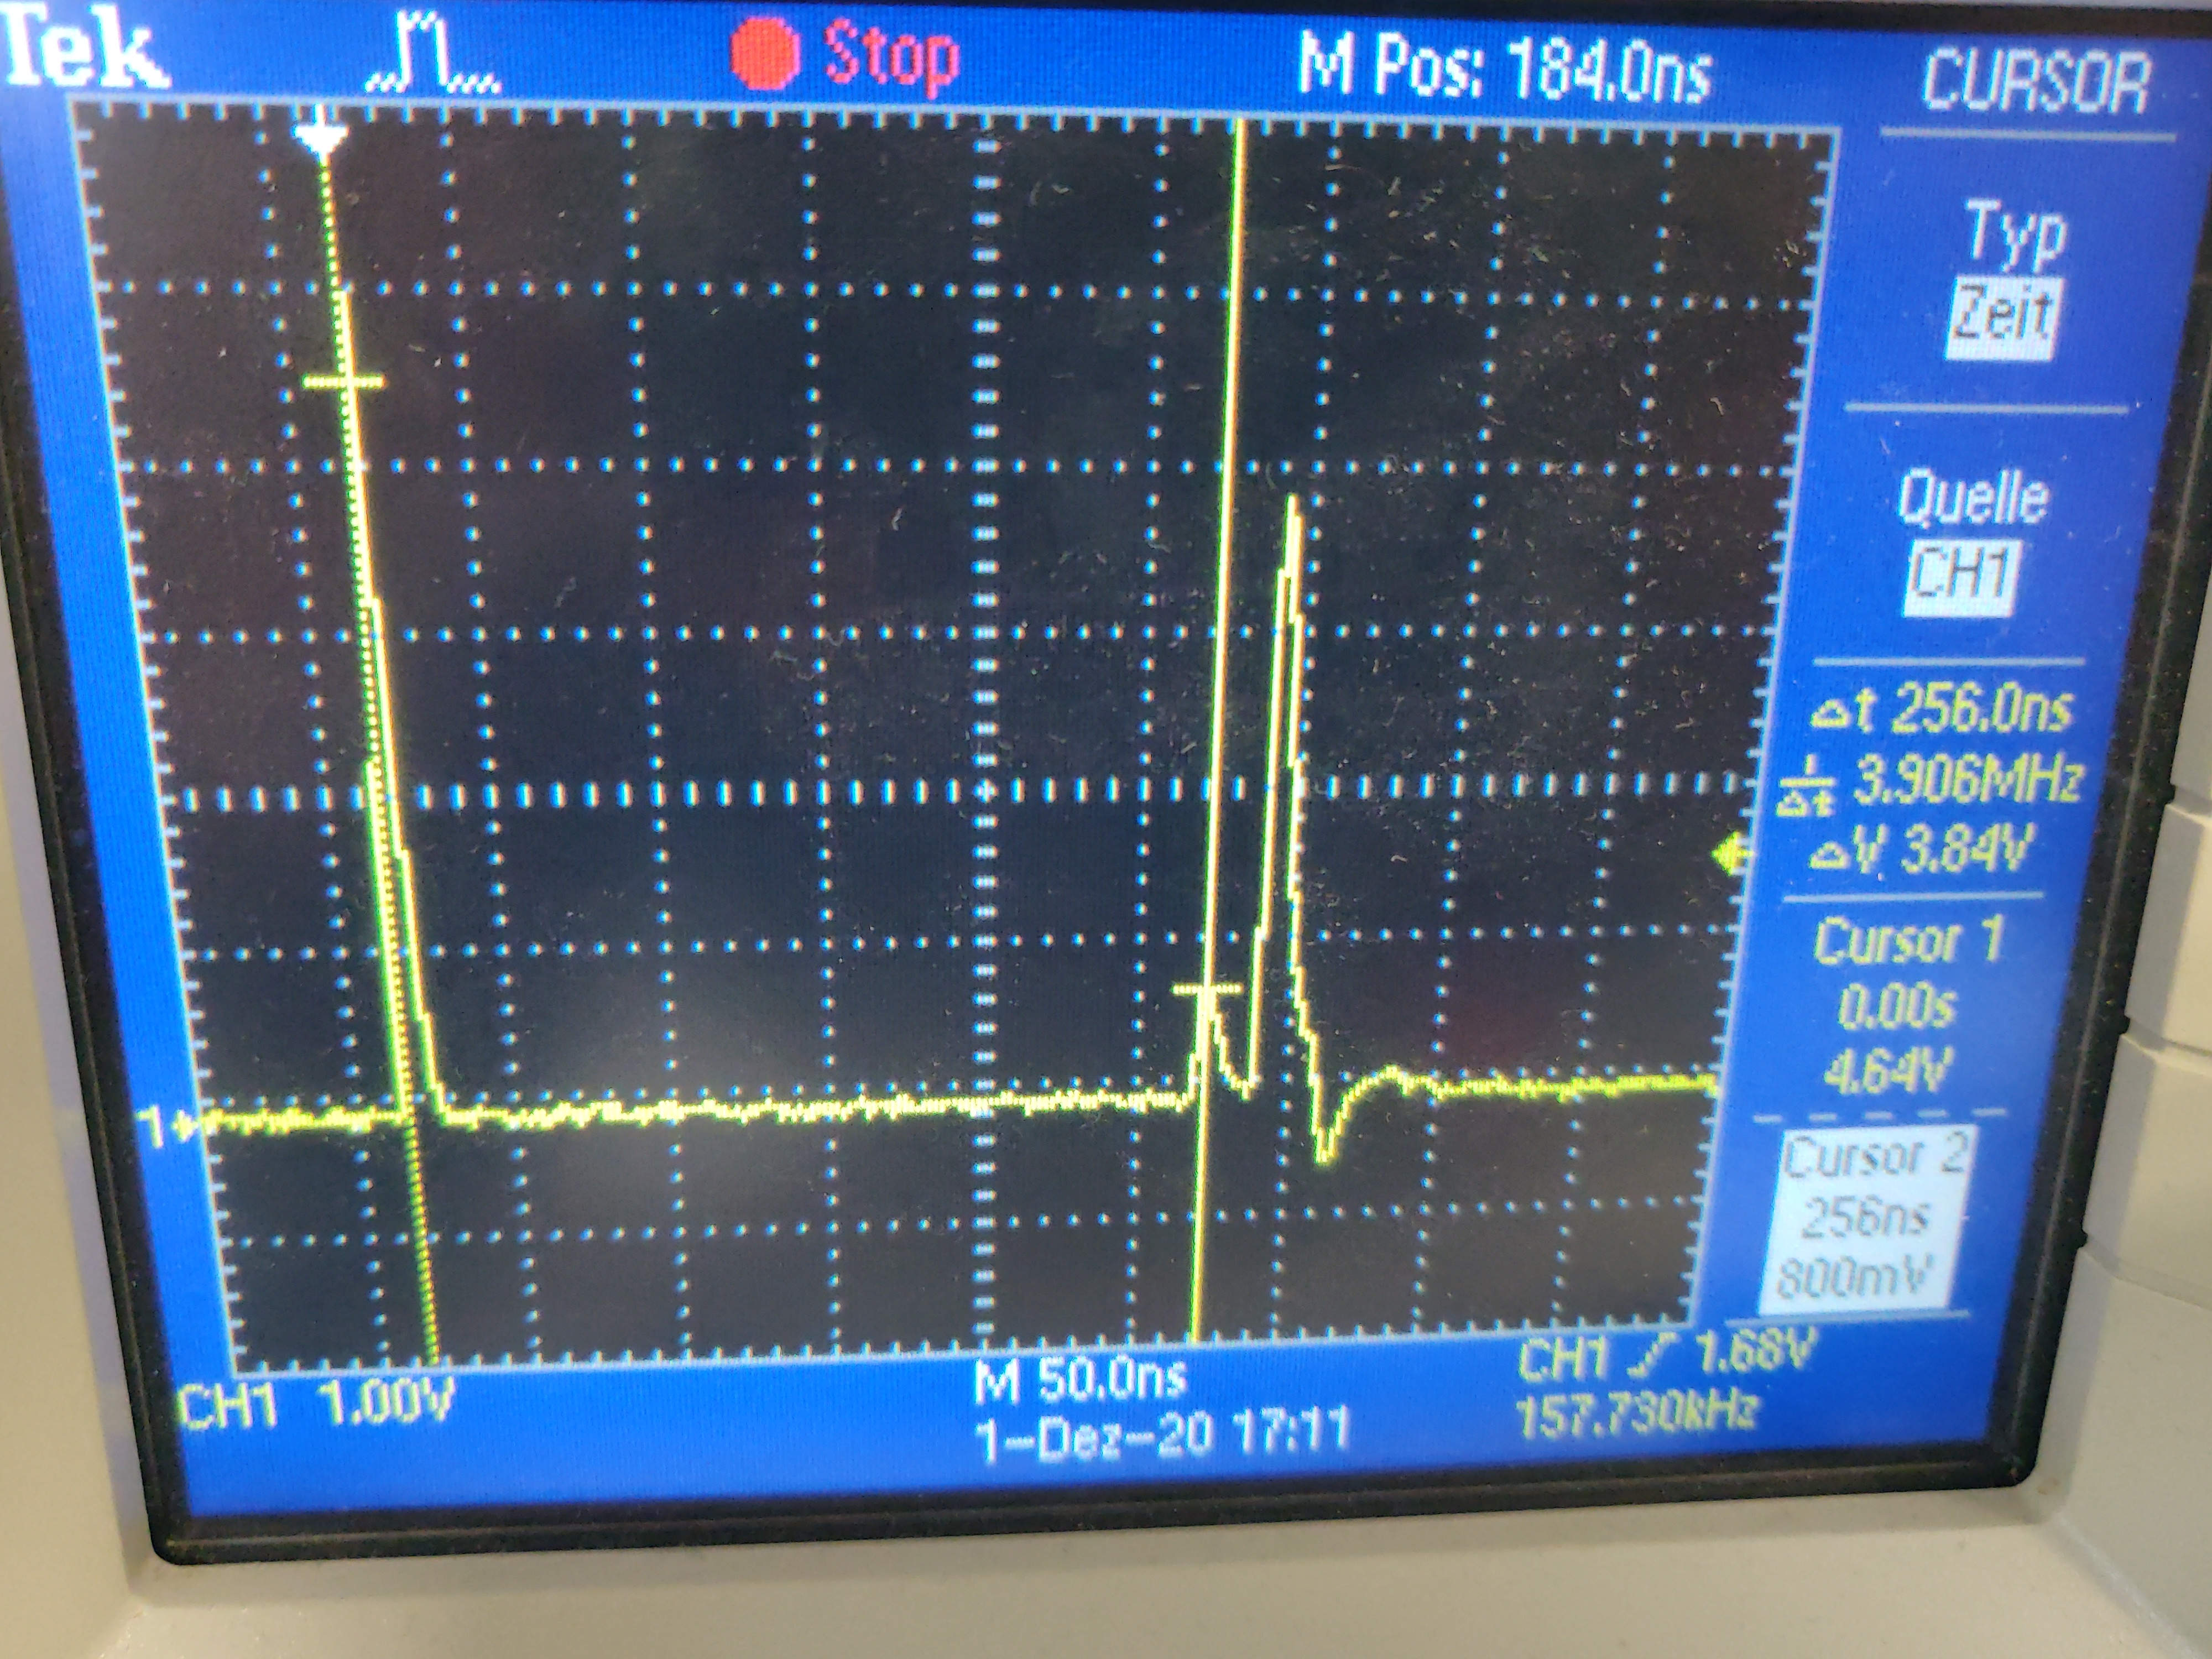
\includegraphics[width=0.45\linewidth]{messdaten/3-3-3_lengthToDefect.jpg}}%
    \hspace{.05\linewidth}
    \subfloat[The length of a transmission line can be deducted by the property of a signal traversing the transmission line at a finite and unaltered speed.\label{subfig:osci:3-3-3_overallLength}]
    {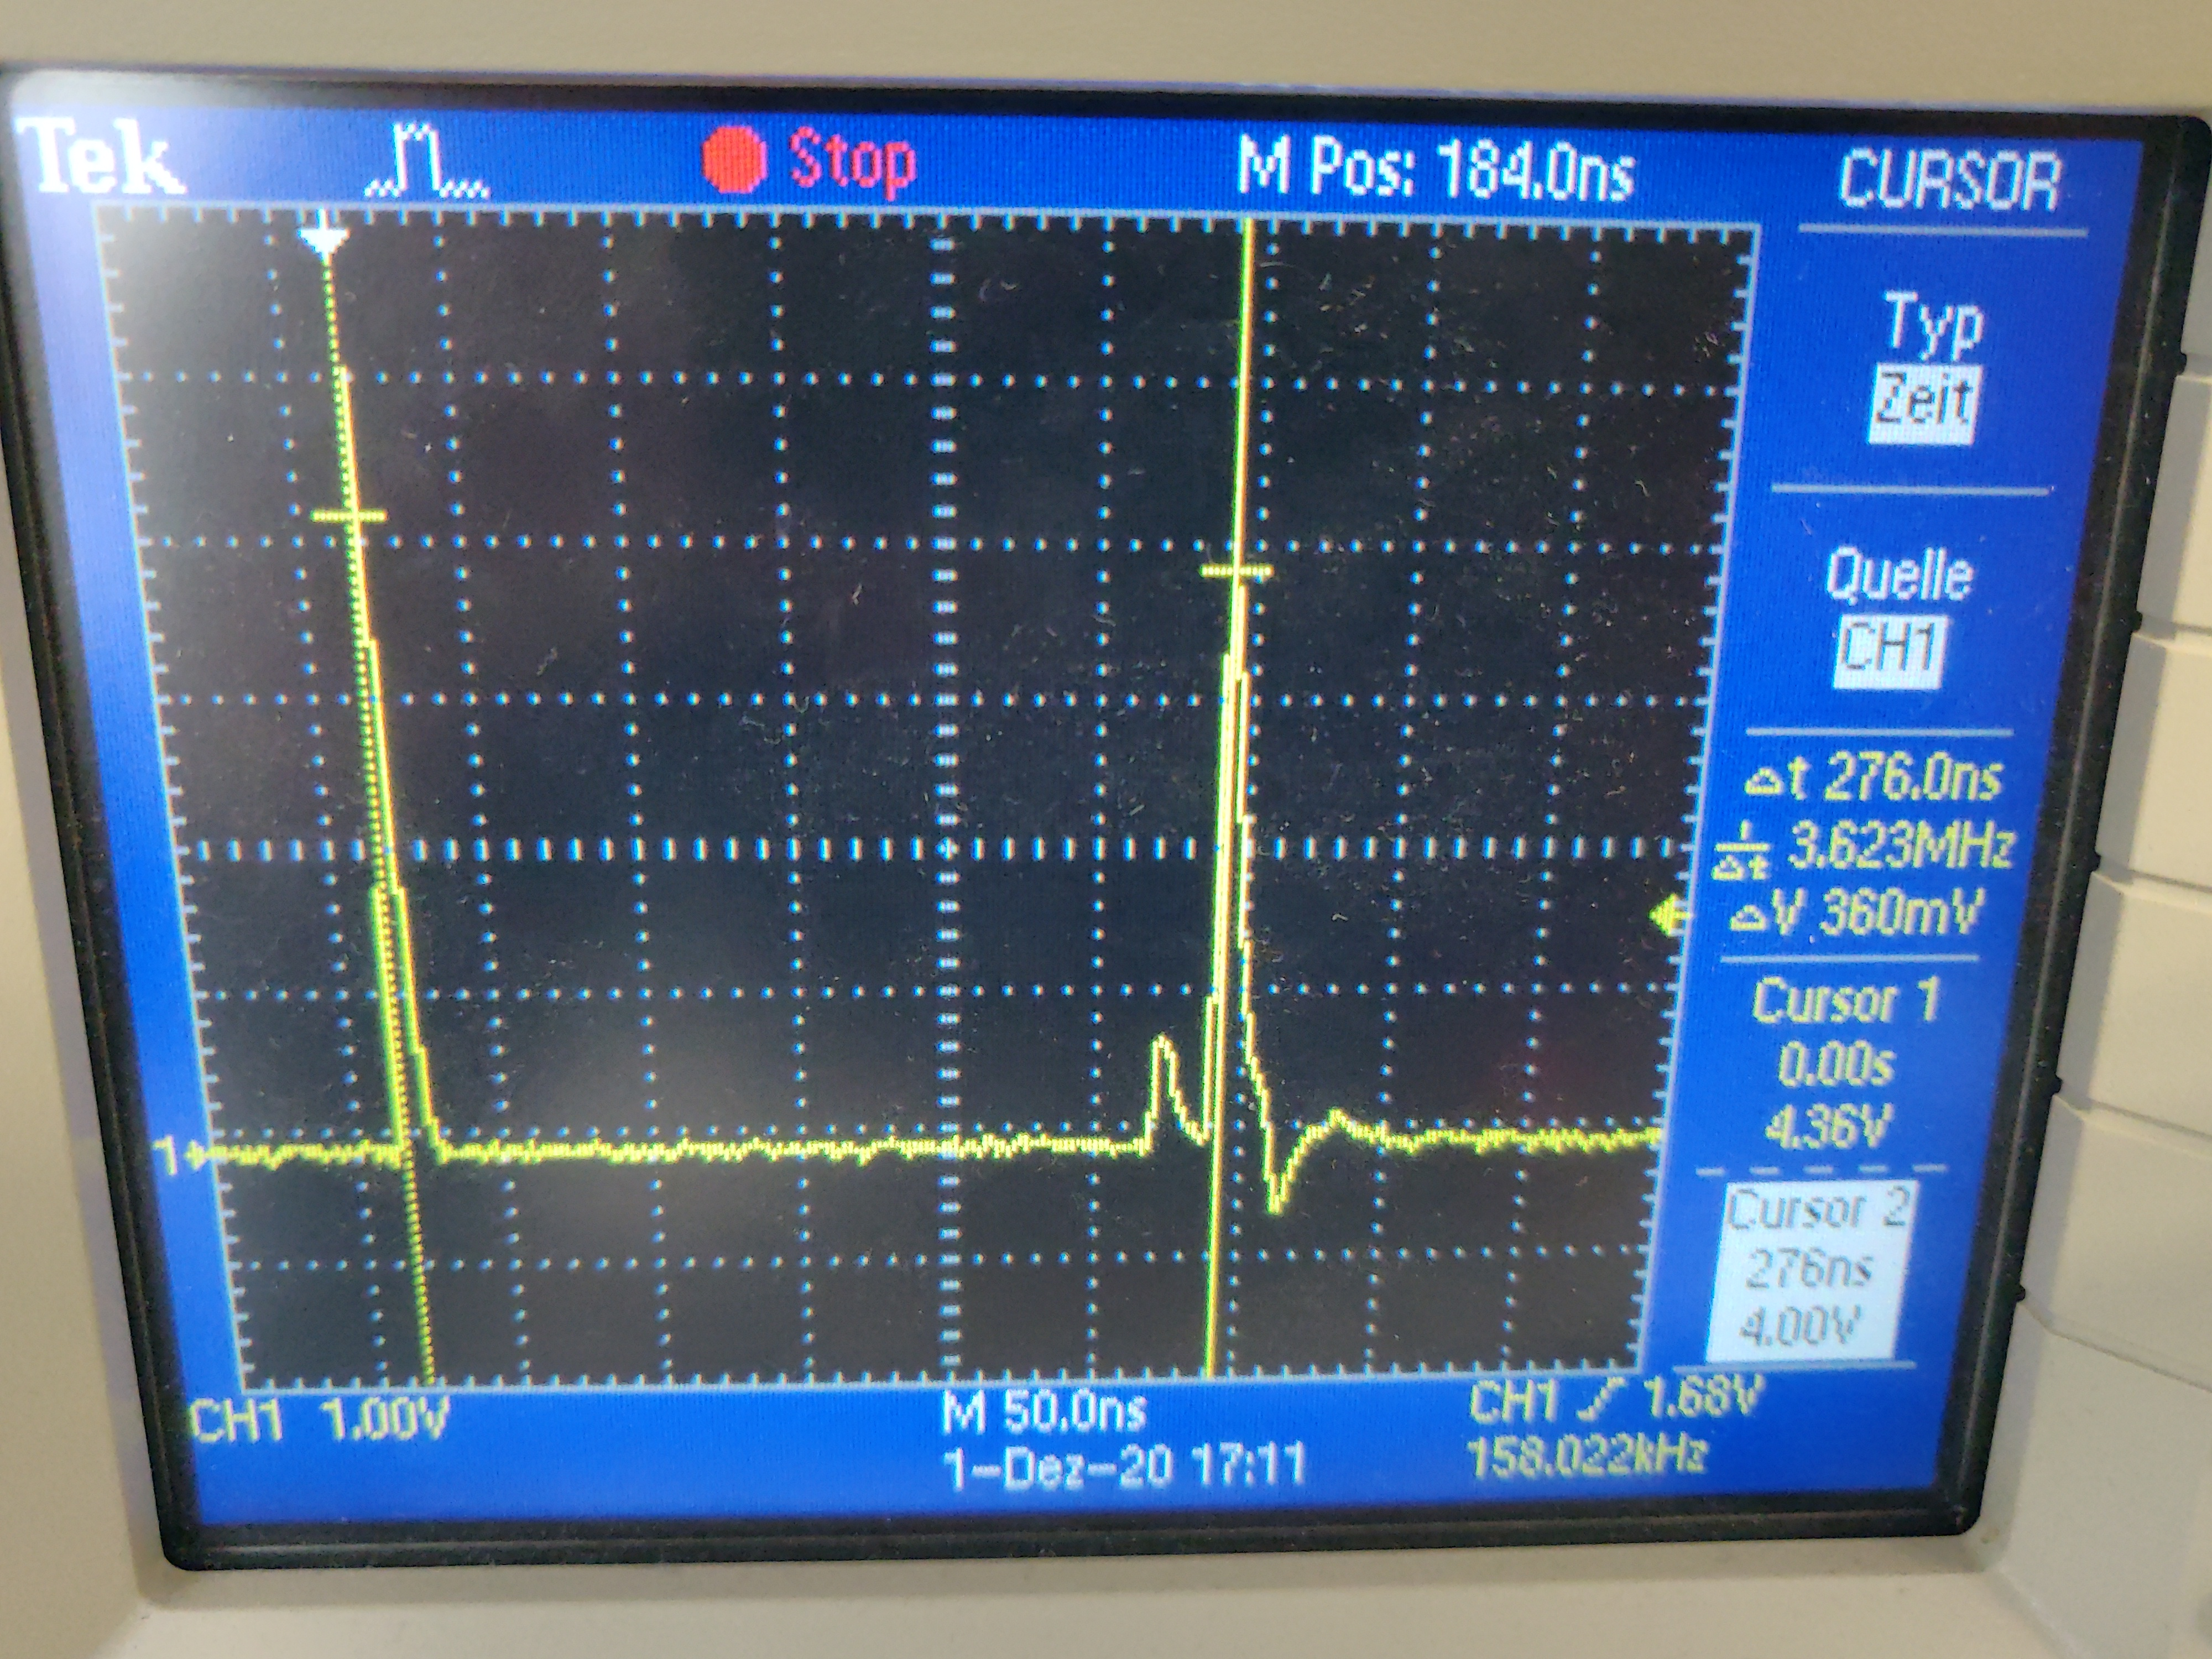
\includegraphics[width=0.45\linewidth]{messdaten/3-3-3_overallLength.jpg}}\\%
    \subfloat[Avalanche pulse signal at $ U_{min} $.\label{subfig:osci:avalanche_pulse_signal}]{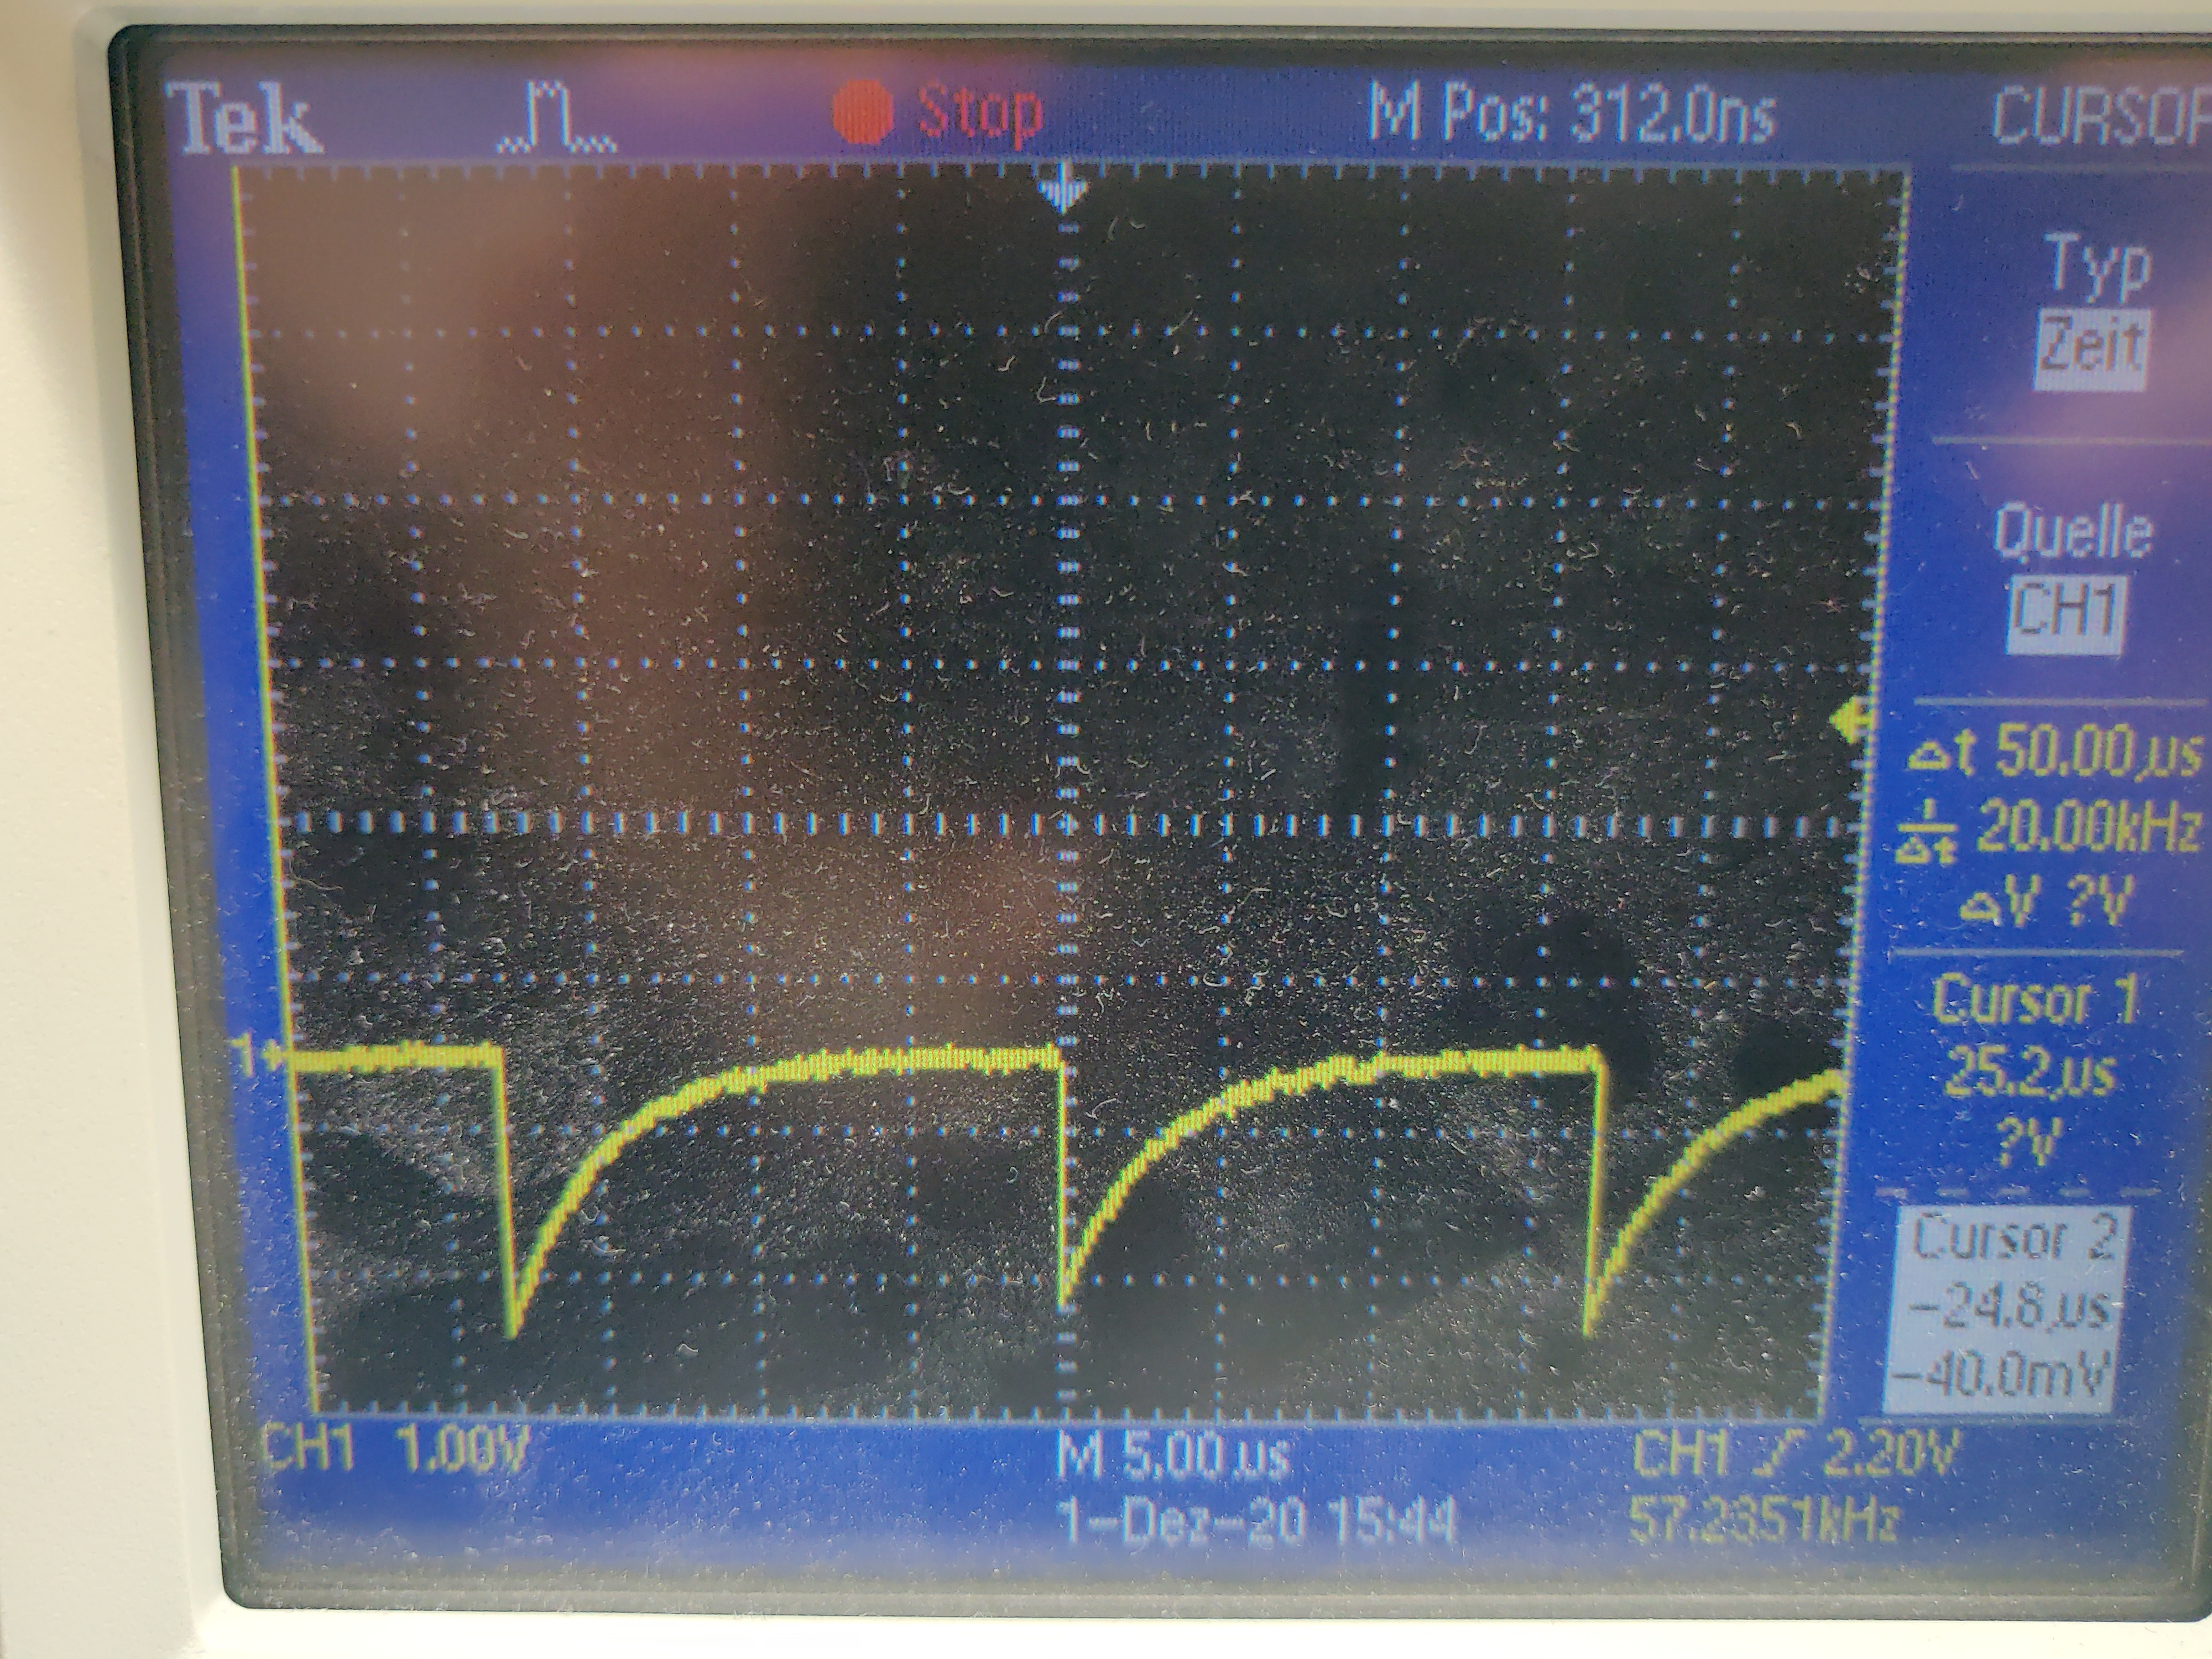
\includegraphics[width=0.45\linewidth]{messdaten/avalanche_pulse_signal.jpg}}%
    \hspace{.05\linewidth}
    \subfloat[Pulse characteristics.\label{subfig:osci:pulsuntersuchung}]{\includegraphics[width=0.45\linewidth]{messdaten/pulsuntersuchung.jpg}}%
    \caption[Oscillograms]{During the course of the experiment captured oscillograms.}%
\end{figure}
%
\begin{figure}
    \centering
    \includesvg[inkscapelatex=false, width=.8\textwidth]{Spice/pulse_attenuation/pulse_attenuation_sim_circuit}
    \caption[\textsc{LTspice} circuit diagram to simulate low-pass behavior]{\textsc{LTspice} circuit diagram to simulate low-pass behavior.}
    \label{fig:pulse_attenuation_sim_circuit}
\end{figure}
%
\newpage
%
\begin{table}[]
    \centering
    \caption[Handwritten notes]{Handwritten notes corresponding each measurement.}%
    \begin{tabular}{cc}
        \adjustbox{valign=t}{
            \subfloat[Duty cycles and measured output voltages at the BC.\label{subtab:3-1_duty_vs_voltage}]{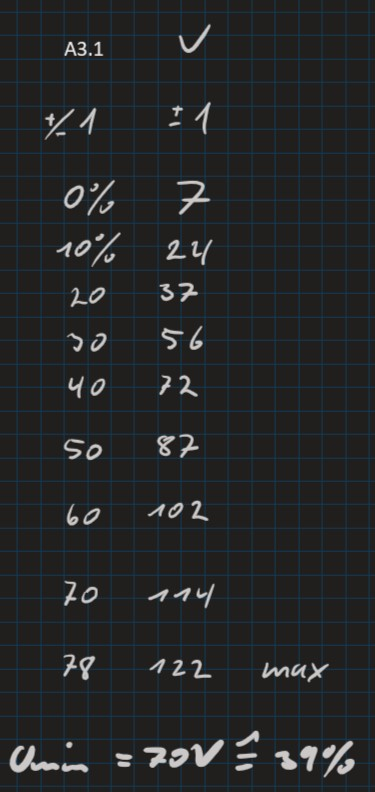
\includegraphics[width=.4\linewidth]{messdaten/handwritten/3-1.jpg}}
            \hspace{.1\linewidth}
        }
        &
        \adjustbox{valign=t}{
            \subfloat[Repetition frequency \( f_{Rep} \) vs. various output voltages.\label{subtab:3-2_duty_vs_repetitionfreq}]{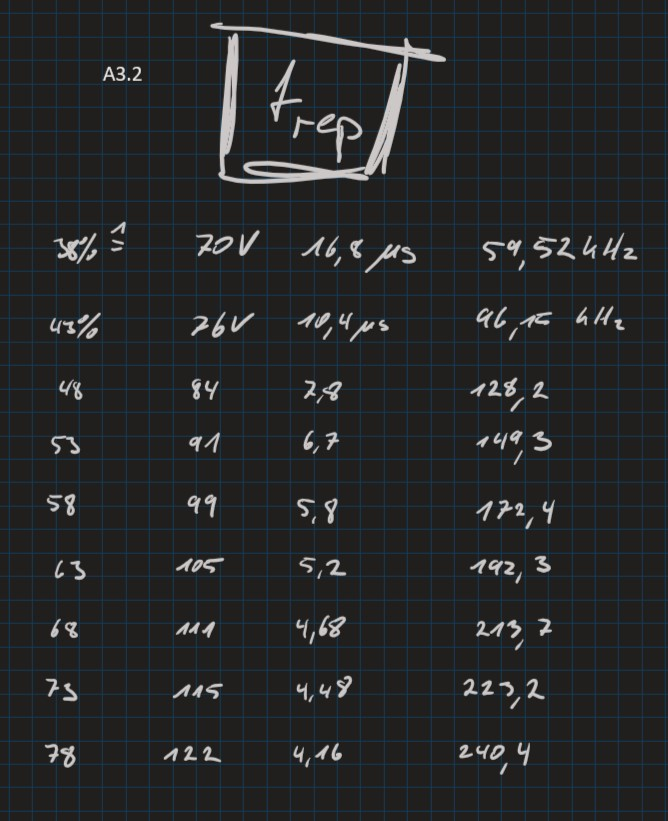
\includegraphics[width=.4\linewidth]{messdaten/handwritten/3-2.jpg}}
            \hspace{.1\linewidth}
        }
    \end{tabular}
\end{table}
\begin{table}[]
    \ContinuedFloat
    \centering
    \begin{tabular}{cc}
        \adjustbox{valign=t}{
            \subfloat[Propagation times at three different cable lengths.\label{subtab:3-3-1_propagationTimes_3_cables}]{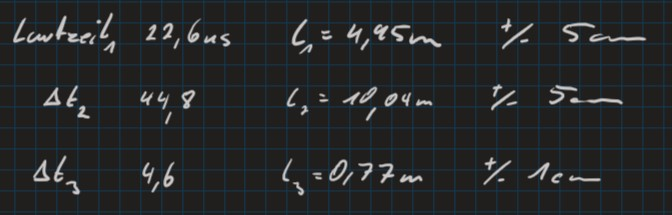
\includegraphics[width=0.4\textwidth]{messdaten/handwritten/3.3.1_propagationTimes.jpg}}%
            \hspace{.1\linewidth}
        }
        &
        \adjustbox{valign=t}{
            \subfloat[Measured impedance of the cables.\label{subtab:3.3.2_cableImpedances}]{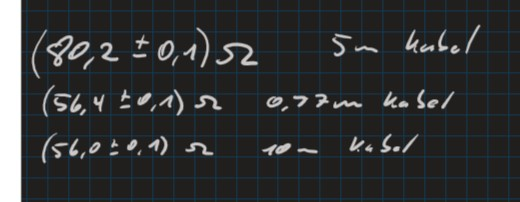
\includegraphics[width=0.4\textwidth]{messdaten/handwritten/3.3.2_cableImpedances.jpg}}%
            \hspace{.1\linewidth}
        }
    \end{tabular}
\end{table}
\begin{table}[]
    \ContinuedFloat
    \centering
    \subfloat[Table of the measured cable characteristics.\label{subtab:3.3.2_cableCharacteristicsTable}]{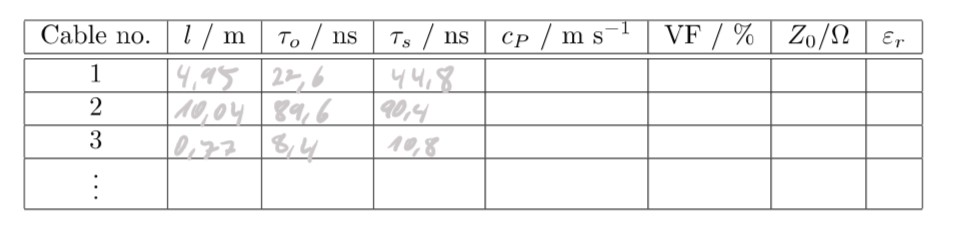
\includegraphics[width=0.6\linewidth]{messdaten/handwritten/3.3.2_cableCharacteristicsTable.jpg}}
\end{table}
%\bibliography{Z:/Dokumente/HSRM/LaTex_Quellen/HSRM_Quellen/quellen}
\printbibliography
%\bibliographystyle{plaindin}
%==========================================
\end{document}